\documentclass[
    article,
    sumario=tradicional,
	% -- opções da classe memoir --
	12pt,				% tamanho da fonte
	openright,			% capítulos começam em pág ímpar (insere página vazia caso preciso)
	oneside,			% para impressão em verso e anverso. Oposto a oneside
	a4paper,			% tamanho do papel. 
	% -- opções da classe abntex2 --
	chapter=TITLE,		% títulos de capítulos convertidos em letras maiúsculas
	section=TITLE,		% títulos de seções convertidos em letras maiúsculas
	subsection=Title,	% títulos de subseções convertidos em letras maiúsculas
	%subsubsection=TITLE,% títulos de subsubseções convertidos em letras maiúsculas
	% -- opções do pacote babel --
	%english,			% idioma adicional para hifenização
	%french,				% idioma adicional para hifenização
	%spanish,			% idioma adicional para hifenização
	brazil				% o último idioma é o principal do documento
	]{abntex2}

\usepackage{ifthen,ifpdf}

\ifpdf
  \pdfpagewidth=\paperwidth
  \pdfpageheight=\paperheight
\fi

% --- 
% CONFIGURAÇÕES DE PACOTES
% --- 
% ---
% Pacotes básicos 
% ---
\usepackage{lmodern}			% Usa a fonte Latin Modern			
\usepackage[T1]{fontenc}		% Selecao de codigos de fonte.
\usepackage[utf8]{inputenc}		% Codificacao do documento (conversão automática dos acentos)
\usepackage{lastpage}			% Usado pela Ficha catalográfica
\usepackage{indentfirst}		% Indenta o primeiro parágrafo de cada seção.
\usepackage{color}				% Controle das cores
\usepackage{graphicx}			% Inclusão de gráficos
\usepackage{microtype} 			% para melhorias de justificação
\usepackage{ufc-abntex2}
\usepackage{enumitem}
\usepackage{amsmath}
\usepackage{booktabs}
\usepackage{multirow}
\usepackage{titlesec}
\usepackage{mathptmx}                               % Usa a fonte Times New Roman
\usepackage{float}
%formatação do Sumário
\usepackage{etoolbox}                               
% Usado para alterar a fonte da Section no Sumário
\usepackage[nogroupskip,nonumberlist,acronym]{glossaries}     \usepackage{listings}    
%\usepackage{tocloft}
\usepackage{pdfpages}

%
% ---
		
% ---
% Pacotes adicionais, usados apenas no âmbito do Modelo Canônico do abnteX2
% ---
\usepackage{lipsum}				% para geração de dummy text
% ---
\usepackage{longtable}
% ---
% Pacotes de citações
% ---
%\usepackage[brazilian,hyperpageref]{backref}	 % Paginas com as citações na bibl
%\usepackage[alf]{abntex2cite}	% Citações padrão ABNT

%Com et al nas referências
%\usepackage[alf, abnt-emphasize=bf, bibjustif, recuo=0cm, abnt-etal-cite=3, abnt-etal-text=it, abnt-etal-list=3]{abntex2cite} 

%Sem et al nas referências
\usepackage[alf, abnt-emphasize=bf, bibjustif, recuo=0cm, abnt-etal-cite=3, abnt-etal-text=it, abnt-etal-list=0]{abntex2cite} 

% Ambiente para alineas e e subalineas (incisos) com ponto
\newlist{alineascomponto}{itemize}{2}
\setlist[alineascomponto,1]{label={$\bullet$},topsep=0pt,itemsep=0pt,leftmargin=\parindent+\labelwidth-\labelsep}%
\setlist[alineascomponto,2]{label={--},topsep=0pt,itemsep=0pt,leftmargin=*}
\newlist{subalineascomponto}{enumerate}{1}
\setlist[subalineascomponto,1]{label={$\circ$},topsep=0pt,itemsep=0pt,leftmargin=*}%
% ---

% Ambiente para alineas e e subalineas (incisos) com numeros
\newlist{alineascomnumero}{enumerate}{2}
\setlist[alineascomnumero,1]{label={$\arabic*$.},topsep=0pt,itemsep=0pt,leftmargin=\parindent+\labelwidth-\labelsep}%
\setlist[alineascomnumero,2]{label={--},topsep=0pt,itemsep=0pt,leftmargin=*}
\newlist{subalineascomnumero}{enumerate}{1}
\setlist[subalineascomnumero,1]{label={$\arabic*$.},topsep=0pt,itemsep=0pt,leftmargin=*}%
% ---

% ---
% Configurações do pacote backref
% Usado sem a opção hyperpageref de backref
%\renewcommand{\backrefpagesname}{Citado na(s) página(s):~}
% Texto padrão antes do número das páginas
%\renewcommand{\backref}{}
% Define os textos da citação
%\renewcommand*{\backrefalt}[4]{
%	\ifcase #1 %
%		Nenhuma citação no texto.%
%	\or
%		Citado na página #2.%
%	\else
%		Citado #1 vezes nas páginas #2.%
%	\fi}%
% ---

% ---
% Configurações de aparência do PDF final

% alterando o aspecto da cor azul
\definecolor{blue}{RGB}{41,5,195}

% informações do PDF
\makeatletter
\hypersetup{
     	%pagebackref=true,
		pdftitle={\@title}, 
		pdfauthor={\@author},
    	pdfsubject={\imprimirpreambulo},
	    pdfcreator={LaTeX with abnTeX2},
		pdfkeywords={abnt}{latex}{abntex}{abntex2}{trabalho acadêmico}, 
		colorlinks=true,       		% false: boxed links; true: colored links
    	linkcolor=blue,          	% color of internal links
    	citecolor=blue,        		% color of links to bibliography
    	filecolor=magenta,      		% color of file links
		urlcolor=blue,
		bookmarksdepth=4
}
\makeatother
% --- 

\makeatletter
\def\@biblabel#1{}
\renewenvironment{thebibliography}[1]
     {\section*{\refname}%
      \@mkboth{\MakeUppercase\refname}{\MakeUppercase\refname}%
      \list{\@biblabel{\@arabic\c@enumiv}}%
           {\settowidth\labelwidth{\@biblabel{#1}}%
            \leftmargin\labelwidth
            %\advance\leftmargin\labelsep
            \@openbib@code
            \usecounter{enumiv}%
            \let\p@enumiv\@empty
            \renewcommand\theenumiv{\@arabic\c@enumiv}}%
      \sloppy
      \clubpenalty4000
      \@clubpenalty \clubpenalty
      \widowpenalty4000%
      \sfcode`\.\@m}
     {\def\@noitemerr
       {\@latex@warning{Empty `thebibliography' environment}}%
      \endlist}
\makeatother

% --- 
% Espaçamentos entre linhas e parágrafos 
% --- 

% O tamanho do parágrafo é dado por:
\setlength{\parindent}{1.5cm}


\setlength{\parindent}{2cm}

% ---
% compila o indice
% ---
\makeindex
% ---


% Define as margens do documento
\setlrmarginsandblock{3cm}{2cm}{*} % externa / interna
\setulmarginsandblock{3cm}{2cm}{*} % superior / inferior

% Define o espaço entre linhas para 1.5 cm
%\OnehalfSpacing	Bug no ABNTEX2?
\renewcommand{\baselinestretch}{1.5}



\usepackage{hyperref}% http://ctan.org/pkg/hyperref
\hypersetup{%
  colorlinks = false,
  linkcolor  = black
}

% Informações de dados para CAPA e FOLHA DE ROSTO
\titulo{Detecção de comentários pejorativos em vídeos infanto-juvenis do Youtube}
\autor{Luiz Isaias de Souza Silva}
\local{Quixadá}
\data{2018}
\orientador{Profª. Dra. Ticiana Coelho da Silva}
%\coorientador{Nome Coorientador}

% Escolher curso: Redes de Computadores (rc), Eng.Software (es), Ciências da Computação (cc) ou Sist.Informação (si)
%\instituicao{%
Universidade Federal do Ceará \par
Campus Quixadá \par
Curso de Redes de Computadores
}

\ies{Universidade Federal do Ceará}
\campus{Campus de Quixadá}
\curso{Curso de Redes de Computadores}

\tipotrabalho{Trabalho de Conclusão de Curso (Monografia)}
\preambulo{Monografia apresentada ao Curso de Redes de Computadores do Campus Quixadá da Universidade Federal do Ceará, como requisito parcial para obtenção do Título de Tecnólogo em Redes de Computadores.}

%\instituicao{%
Universidade Federal do Ceará \par
Campus Quixadá \par
Curso de Sistemas de Informação
}

\ies{Universidade Federal do Ceará}
\campus{Campus de Quixadá}
\curso{Curso de Sistemas de Informação}

\tipotrabalho{Trabalho de Conclusão de Curso (Monografia)}
\preambulo{Monografia apresentada ao Curso de Sistemas de Informação do Campus Quixadá da Universidade Federal do Ceará, como requisito parcial para obtenção do Título de Bacharel em Sistemas de Informação.}

\instituicao{
Universidade Federal do Ceará \par
Campus de Quixadá \par
Curso de Engenharia de Software
}

\ies{Universidade Federal do Ceará}
\campus{Campus de Quixadá}
\curso{Curso de Engenharia de Software}

\tipotrabalho{Trabalho de Conclusão de Curso (Monografia)}
\preambulo{Monografia apresentada ao Curso de Engenharia de Software do Campus Quixadá da Universidade Federal do Ceará, como requisito parcial para obtenção do Título de Bacharel em Engenharia de Software.}

%\instituicao{%
Universidade Federal do Ceará \par
Campus Quixadá \par
Curso de Ciência da Computação
}


\ies{Universidade Federal do Ceará}
\campus{Campus de Quixadá}
\curso{Curso de Ciência da Computação}

\tipotrabalho{Trabalho de Conclusão de Curso (Monografia)}
\preambulo{Monografia apresentada ao Curso de Ciências da Computação do Campus Quixadá da Universidade Federal do Ceará, como requisito parcial para obtenção do Título de Bacharel em Ciências da Computação.}
 

%%criar um novo estilo de cabeçalhos e rodapés
\makepagestyle{header_style}
  %%cabeçalhos
  \makeoddhead{header_style} %%pagina ímpar ou com oneside
     {}
     {}
     {\thepage} 


\begin{document}
\frenchspacing 

%Formatação de título de seções
\titleformat{\section}
{\normalfont\normalsize\bfseries}{\thesection}{1em}{}
\titleformat{\subsection}
{\normalfont\normalsize\bfseries}{\thesubsection}{1em}{}
\titleformat{\subsubsection}
{\normalfont\normalsize\bfseries}{\thesubsubsection}{1em}{}

\renewcommand{\cftsectionfont}{\normalfont\normalsize}   
\renewcommand{\cftsubsectionfont}{\normalfont\normalsize} 
\renewcommand{\cftsubsubsectionfont}{\normalfont\normalsize}  

% ----------------------------------------------------------
% ELEMENTOS PRÉ-TEXTUAIS
% ----------------------------------------------------------
% \pretextual
% Capa
\imprimircapa

%----------- Apenas TCC 2
% Folha de rosto (* indica que haverá a ficha bibliográfica)
\imprimirfolhaderosto

% Ficha Bibliográfica
% ---
% Inserir a ficha bibliografica
% ---

% Isto é um exemplo de Ficha Catalográfica, ou ``Dados internacionais de
% catalogação-na-publicação''. Você pode utilizar este modelo como referência. 
% Porém, provavelmente a biblioteca da sua universidade lhe fornecerá um PDF
% com a ficha catalográfica definitiva após a defesa do trabalho. Quando estiver
% com o documento, salve-o como PDF no diretório do seu projeto e substitua todo
% o conteúdo de implementação deste arquivo pelo comando abaixo:
%
\begin{fichacatalografica}
    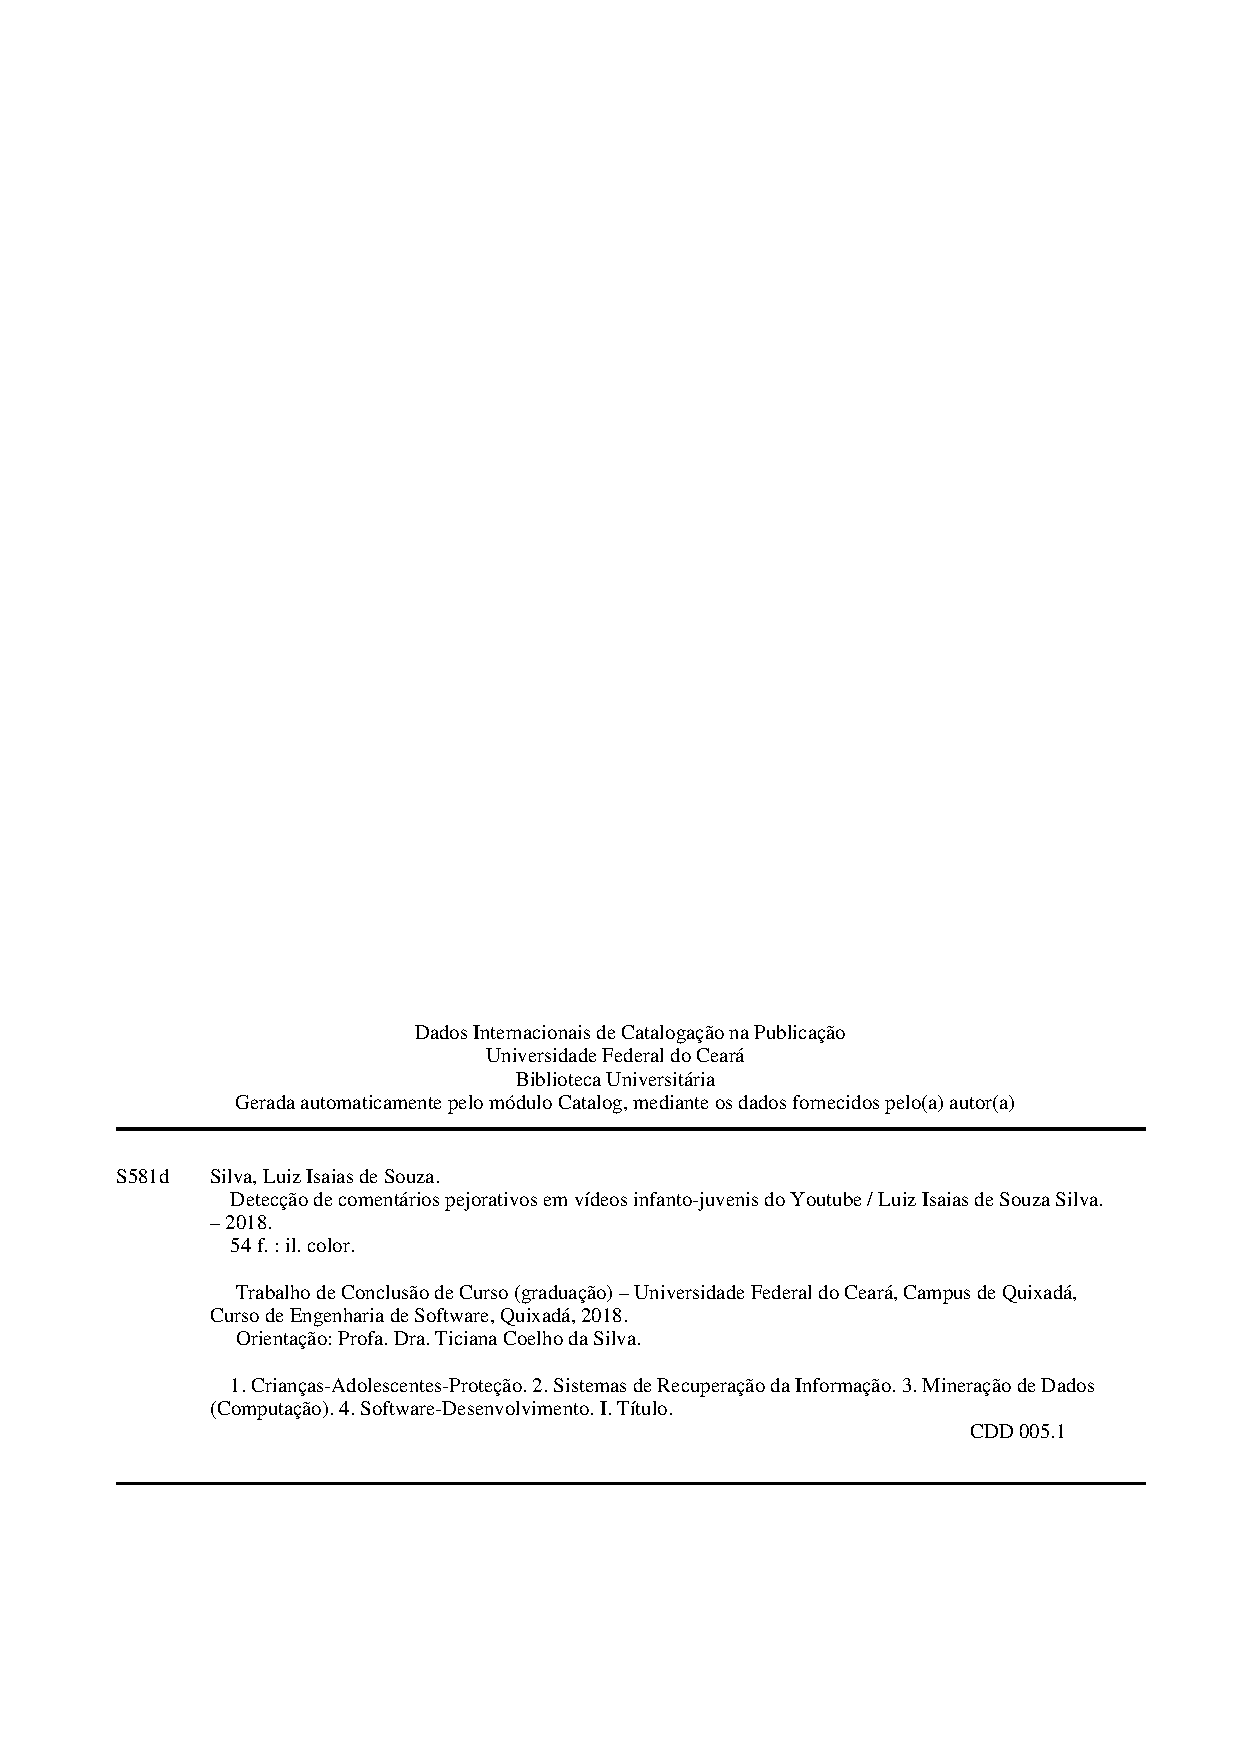
\includepdf[pages=1]{ficha.pdf}
\end{fichacatalografica}

% ---

% Errata
%% ---
% Inserir errata
% ---
\begin{errata}
Elemento opcional da NORMA. Exemplo:

\vspace{\onelineskip}

FERRIGNO, C. R. A. \textbf{Tratamento de neoplasias ósseas apendiculares com
reimplantação de enxerto ósseo autólogo autoclavado associado ao plasma
rico em plaquetas}: estudo crítico na cirurgia de preservação de membro em
cães. 2011. 128 f. Tese (Livre-Docência) - Faculdade de Medicina Veterinária e
Zootecnia, Universidade de São Paulo, São Paulo, 2011.

\begin{table}[htb]
\center
\footnotesize
\begin{tabular}{|p{1.4cm}|p{1cm}|p{3cm}|p{3cm}|}
  \hline
   \textbf{Folha} & \textbf{Linha}  & \textbf{Onde se lê}  & \textbf{Leia-se}  \\
    \hline
    1 & 10 & auto-conclavo & autoconclavo\\
   \hline
\end{tabular}
\end{table}

\end{errata}
% ---


% Folha de Aprovação
% DEVE ser modificada para adicionar os membros da banca
% ---
% Inserir folha de aprovação
% ---

% Isto é um exemplo de Folha de aprovação, elemento obrigatório da NBR
% 14724/2011 (seção 4.2.1.3). Você pode utilizar este modelo até a aprovação
% do trabalho. Após isso, substitua todo o conteúdo deste arquivo por uma
% imagem da página assinada pela banca com o comando abaixo:
%
% \includepdf{folhadeaprovacao_final.pdf}
%
\begin{folhadeaprovacao}

    \begin{center}
		\MakeUppercase{\imprimirautor}\par
		\vspace{\onelineskip}
	    \vspace{2cm}
		\vspace{\onelineskip}
		\MakeUppercase{\imprimirtitulo}
	\end{center}

    \vspace{\onelineskip}
	\vspace{2cm}
	\vspace{\onelineskip}
	
	%Retira o espaco do paragrafo
	\hspace*{-2cm}
	%Adiciona o espaço da margem
	\hspace*{8cm}	
	\begin{minipage}{8cm}
		\begin{SingleSpace}
			\imprimirpreambulo \\			
		\end{SingleSpace}		
	\end{minipage}

	\vspace{\onelineskip}
		
	\noindent Aprovada em: \_\_/\_\_/\_\_\_\_
	
	\vspace{\onelineskip}
     
    \vspace{2cm}
	\textbf{BANCA EXAMINADORA}
   
	

   \assinatura{\imprimirorientador \space (Orientadora) \\ Universidade Federal do Ceará (UFC)}
   %\assinatura{\imprimircoorientador \space (Co-Orientador) \\ Universidade Federal do Ceará (UFC)}
   %DEFINA AQUI OS DEMAIS MEMBROS DA BANCA
   \assinatura{Prof. Me. Regis Pires Magalhães \\ Universidade Federal do Ceará (UFC)}
   \assinatura{Prof. Dra. Carla Ilane Moreira Bezerra \\ Universidade Federal do Ceará (UFC)}
   %\assinatura{Prof. Msc. Livia Almada \\ Universidade Federal do Ceará (UFC)}
      
%   \begin{center}
%    \vspace*{0.5cm}
%    {\large\imprimirlocal}
%    \par
%    {\large\imprimirdata}
%    \vspace*{1cm}
%  \end{center}
  
\end{folhadeaprovacao}
% ---

%\imprimirfolhadeaprovacao

% Dedicatória
% ---
% Dedicatória
% ---
\begin{dedicatoria}
   \vspace*{\fill}
   	\begin{flushright}
   \noindent
    Ao meu pai Luiz Claudio.\\
    À Minha mãe Pergentina Rodrigues.\\
    À todos da minha família que me deram apoio e acreditaram.\\
    Aos meus amigos de longa data em Fortaleza, aos novos amigos que fiz em Quixadá, e à todos que virão.
   	\end{flushright}
\end{dedicatoria}
% ---

% Agradecimentos
% ---
% Agradecimentos
% ---

\begin{center}
	\bfseries\MakeUppercase{AGRADECIMENTOS}\par
\end{center}
	
Primeiramente gostaria de dedicar esse trabalho à minha Mãe, por ter dado seu sangue para que que eu pudesse chegar onde cheguei, me provendo uma educação básica de qualidade, cursos e preparação para o futuro. Apesar de nossas diferenças em pensamento e atitude, saiba que eu te amo do fundo do meu coração, e eu jamais estaria aqui se não fosse por você. Quero sempre ter os motivos para continuar te orgulhando.

Ao meu pai que sempre me orientou e me educou sobre a vida. Me ajudou a descobrir minha grande paixão, que é programação, me mostrou o que é ter de "se virar", e me mostrou o quanto é bom ter liberdade e caminhar com as próprias pernas. Você é meu modelo, principalmente para as atitudes boas e nobres. Eu jamais teria tido a força e a coragem para sair de casa, se não fosse por você. Agora o céu é o limite!

À todos da minha família que me apoiaram, em especial meus padrinhos e meus irmãos e minha avó D. Teresa.

Um "muito obrigado!" especial para a pessoa que me aturou, mesmo com minhas crises e inconstâncias, e me mostrou o que é amar e ser amado durante os últimos 4 anos, Letícia Aguiar, você foi e sempre será alguém especial, e apesar de termos de seguir caminhos diferentes, saiba que o que sinto é verdadeiro e apesar de não ser imortal, visto que é chama, é eterno enquanto durar. % Sim, é vinicius de moraes

Aos meus amigos que ficaram e à todos os amigos que fiz em Quixadá, em especial Caio Melo, Gabriel Jorge, Ana Carmélia, Gustavo Carneiro, Sérgio Gadelha, Matheus Rios, Bruna Kelvyla, Adson Rodrigues e Felipe Souza.

Eu acredito que uma pessoa pode sempre evoluir e chegar numa versão melhor de si mesmo. Basta crer em suas atitudes e na sua capacidade, e sempre buscar melhorar.

Em memória do meu eterno melhor amigo, Gohan.
% ---
%\imprimiragradecimentos{editaveis/agradecimentos}

% Epígrafe
% ---
% Epígrafe
% ---
\begin{epigrafe}
    \vspace*{\fill}
	\begin{flushright}
		\textit{``A gente destrói aquilo que mais ama\\
em campo aberto, ou numa emboscada;\\
alguns com a leveza do carinho\\
outros com a dureza da palavra;\\
os covardes destroem com um beijo\\
os valentes destroem com a espada.\\
		(Oscar Wilde, A Balada do Cárcere de Reading)}
	\end{flushright}
\end{epigrafe}
% ---

% RESUMOS
%% resumo em português

%\begin{resumoo}

\setlength{\absparsep}{18pt} % ajusta o espaçamento dos parágrafos do resumo

\begin{resumo}[\normalfont\normalsize\bfseries\MakeUppercase RESUMO]
 A Internet, rede mundial de computadores, conecta cada vez mais pessoas ao redor do mundo. Em um dos sites mais acessados do mundo, a plataforma de vídeos Youtube, é notável a participação ativa de jovens e crianças nos comentários dos vídeos. Também é notável a quantidade de ofensas direcionadas aos usuários, nesses comentários. Quando os vídeos são direcionados às crianças e adolescentes, isso pode influenciar negativamente os jovens e ferir o Estatuto da Criança e do Adolescente brasileiro que afirma: "Deve ser respeitado a integridade física, moral e psíquica da criança e do adolescente". 
 Com o objetivo de detectar se um vídeo no Youtube, direcionado aos jovens, possui muitos comentários negativos desenvolvemos um classificador textual Naïve Bayes e uma extensão para o navegador Google Chrome, que indica a taxa de comentários pejorativos contidos no vídeo.
 Para analisar comentários de vídeos do Youtube e montar o modelo de classificação textual, foram utilizadas ferramentas de mineração e classificação de dados NLTK, scikit-learn e SentiStrength. Para auxiliar e automatizar os passos de coleta e extração dos comentários de vídeos do Youtube, o autor desenvolveu vários scripts na linguagem Python. Uma extensão para Google Chrome foi desenvolvida, utilizando tecnologias web, para aproveitar os dados de classificação gerados, e facilitar a realização de novas classificações.
 Ao total, 87.094 comentários foram coletados, e 62.121 foram analisados, apresentando 48.773 comentários considerados neutros e 13.348 comentários considerados pejorativos.
 Observou-se que vídeos direcionados à crianças não possuem altas taxas de comentários negativos, e por outro lado, vídeos direcionados a jovens, possuem uma taxa de 34\% de comentários pejorativos, ou seja vídeos direcionados à adolescentes possuem mais termos ofensivos em seus comentários.
 

 \textbf{Palavras-chaves}: Sistema de Recuperação da Informação. Mineração de Dados. Proteção de Crianças e Adolescentes.
\end{resumo}
%\end{resumoo}
%% resumo em inglês
\begin{resumo}[Abstract]
 \begin{otherlanguage*}{english}
   This is the english abstract.

   \vspace{\onelineskip}
 
   \noindent 
   \textbf{Key-words}: latex. abntex. text editoration.
 \end{otherlanguage*}
\end{resumo}
%% resumo em francês 
\begin{resumo}[Résumé]
 \begin{otherlanguage*}{french}
    Il s'agit d'un résumé en français.
 
   \textbf{Mots-clés}: latex. abntex. publication de textes.
 \end{otherlanguage*}
\end{resumo}

%% resumo em espanhol
\begin{resumo}[Resumen]
 \begin{otherlanguage*}{spanish}
   Este es el resumen en español.
  
   \textbf{Palabras clave}: latex. abntex. publicación de textos.
 \end{otherlanguage*}
\end{resumo}
% ---

% Lista de ilustrações
%\pdfbookmark[0]{\listfigurename}{lof}
%\listoffigures*
%\clearpage
\renewcommand*\listfigurename{\normalfont\normalsize\bfseries Lista de Ilustrações}
\imprimirlistadeilustracoes

% Lista de tabelas
\renewcommand*\listtablename{\normalfont\normalsize\bfseries Lista de Tabelas}
\pdfbookmark[0]{\listtablename}{lot}
\listoftables*
\cleardoublepage

% Abreviaturas e Siglas
%% Lista de abreviaturas e siglas
% ---
\begin{siglas}
  \item[ABNT] Associação Brasileira de Normas Técnicas
  \item[abnTeX] ABsurdas Normas para TeX
\end{siglas}
% ---

% Símbolos
%%Lista de símbolos
% ---
\begin{simbolos}
  \item[$ \Gamma $] Letra grega Gama
  \item[$ \Lambda $] Lambda
  \item[$ \zeta $] Letra grega minúscula zeta
  \item[$ \in $] Pertence
\end{simbolos}
% ---
%----------- fim - Apenas TCC 2


% Sumário

\imprimirsumario

% ----------------------------------------------------------
% ELEMENTOS TEXTUAIS
% ----------------------------------------------------------
\textual

%aplicação de estilo de cabeçalho
\pagestyle{header_style}

%uso do input pois o include dá quebra de página no final
\section{INTRODUÇÃO}


A internet é uma rede mundial que interliga milhões de computadores em todo o mundo, servindo como um grande fator de comunicação e integração social \cite{marioFalcao2015}. Todo os dias, novas páginas na internet surgem, sejam de relacionamento, humor, entretenimento, notícias, ou redes sociais, como exemplo: Facebook, Twitter, Instagram, Google+, Vimeo, DailyMotion e Youtube.

É pertinente que em nossa sociedade contemporânea, as pessoas estejam mais próximas da tecnologia, principalmente as crianças. 
Essas crianças adquirem habilidades diferentes das crianças de antigamente: enquanto uma criança da década de 80 possuía uma maior facilidade para construir ou modelar um brinquedo, as crianças da geração atual possuem habilidades para lidar com a informática, devido ao convívio rotineiro com a mesma \cite{marioFalcao2016}.

% Motivação para utilização do Youtube
A plataforma de vídeos Youtube é o segundo site mais acessado do mundo \cite{alexaYoutube}. Em tal plataforma, é possível postar e compartilhar vídeos com uma enorme e abrangente gama de conteúdos, servindo também como site de buscas. É possível encontrar conteúdo musical, \textit{vlogs}, animações, curta-metragens, conteúdo educativo, conteúdo com público alvo adulto e conteúdo voltado especificamente ao público jovem e infantil. 

Como parte de suas características de rede social, o Youtube disponibiliza, em seus vídeos, a possibilidade de usuários comentarem. Porém tendo em vista as crianças e adolescentes estão conectadas na rede cada vez mais cedo \cite{EnyoGoncalves2017}, ao navegar pela plataforma, em vídeos infantis nota-se que há uma certa liberdade para realizar comentários de qualquer natureza, até mesmo ofensivos ou inapropriados para o público o qual o vídeo é destinado, um exemplo disso pode ser visto na Figura \ref{fig:youtube_comment}.

% Qual a problemática dos comentários negativos em vídeos infantis. Era bom ter referências de artigos para isso. % ainda n achei
% solution -> ECA
Segundo o artigo 17 do \textbf{Estatuto da Criança e do Adolescente} (ECA): "O direito ao respeito consiste na inviolabilidade da integridade física, psíquica e moral da criança e do adolescente, abrangendo a preservação da imagem, da identidade, da autonomia, dos valores, ideias e crenças, dos espaços e objetos pessoais." \cite{eca_lei}.  Assim, é possível através da tecnologia buscar meios para proteger moralmente e psiquicamente o público mais jovem que utiliza a plataforma. %Esse final não ta legal %

\begin{figure}[H] %use h para forçar que a figura fique abaixo do texto
	\caption{\label{fig:youtube_comment} Comentário do Youtube}
	\begin{center}
	    
\includegraphics[scale=1]{figuras/figura_1.png} % altere o atributo scale para o tamanho da figura
	\end{center}
	\legend{Fonte: Youtube - 13 de Setembro de 2017}
%Verificar se precisa por a data aqui 
\end{figure}

A Figura \ref{fig:youtube_comment} foi retirada do vídeo \textbf{UPA CAVALINHO - Clipe Música Oficial - Galinha Pintadinha DVD 4}, um vídeo direcionado à crianças de 2 a 7 anos postado pelo canal \emph{Galinha Pintadinha}, que é direcionado ao público infantil. %Explicar o comentário que pode ser visualizado e interpretado pela criança. Também seria bom referências para isso. %N.A. (28nov2017) não encontrei referências para "crianças palavrão"; checar os links abaixo:
%http://onlinelibrary.wiley.com/doi/10.1111/j.1365-2214.2011.01338.x/full
%http://www.tandfonline.com/doi/abs/10.1080/01434630408666529
%procurar tb por children+swear words.


Dessa forma, o problema abordado neste trabalho é identificar comentários pejorativos semelhantes ao apresentado na Figura \ref{fig:youtube_comment} em vídeos infantis postados no Youtube. Para solucionar tal problema, primeiramente será utilizada uma ferramenta própria para coleta dos comentários, seguido da utilização de técnicas de mineração de dados, e técnicas de classificação e análise dos dados. Um modelo será elaborado a fim de apontar os comentários pejorativos dos vídeos infantis, podendo assim, ser utilizado para futuramente elaborar meios de alertar os responsáveis e os pais sobre o nível de segurança dos vídeos que estão sendo exibidos às crianças. O modelo também poderá ser aplicado em qualquer vídeo do Youtube.  % Como tu vai fazer isso? Tem que explicar aqui. Para que? O que tu vai fazer com esses comentários? Soluções para denunciar os comentários.
% Para que e para quem  esse estudo vai servir? Escrever um parágrafo sobre isso.

\textcolor{red}{nada do plugin foi mencionado,pq??}

%Falar das ferramentas que serão utilizadas

%\begin{itemize}
 %   \item Questão de Pesquisa?
  %  \item Questão de Pesquisa? 
   % \item Questão de Pesquisa?
%\end{itemize}

%Neste trabalho o idioma dos textos analisados é estritamente português, e na Seção 5 serão esclarecidos os critérios que são considerados para que um comentário seja classificado como pejorativo.

Este trabalho está estruturado da seguinte forma. No Capítulo 2, serão apresentados os principais trabalhos relacionados, que tratam dos temas de mineração e de proteção de crianças online; No Capítulo 3, são apresentados os objetivos do trabalho; No Capítulo 4, são apresentados os principais conceitos que são utilizados durante o projeto; O Capítulo 5 apresenta a metodologia de trabalho; e o Capítulo 6 apresenta \textcolor{blue}{dados preliminares da pesquisa.}

\textcolor{red}{não deveria ser os resultados?}

\textcolor{red}{mover objetivos e fundamentacao teorica para depois da introdução}



\newpage
\section{OBJETIVOS}

Afim de concretizar os resultados desse trabalho, os seguintes objetivos foram estabelecidos.

\subsection{Objetivo Geral}

%Classificar comentários pejorativos em vídeo infantis na plataforma Youtube e avaliar a eficácia desta classificação.
Elaborar um modelo de classificação textual, que classifica se um comentário é apropriado ou não para crianças e adolescentes.
%modelo de que?

\begin{comment}
Example inline comment
\end{comment}

\subsection{Objetivos específicos}

\begin{alineas}
    
    \item Classificar os comentários pejorativos em vídeos infantis do Youtube;
    \item Analisar os comentários classificados;
    \item Indicar os vídeos que possuem mais comentários pejorativos para que os pais protejam seus filhos na plataforma Youtube; 
    \item Avaliar o modelo de classificação proposto;
    \item Desenvolvimento de uma extensão para o navegador da web Google Chrome que permite a visualização dos resultados das classificações realizadas.
    
\end{alineas}


\newpage
\section{FUNDAMENTAÇÃO TEÓRICA}

A seguir, serão detalhados os principais conceitos envolvidos e utilizados durante este trabalho.


%Mineração de textos
\subsection{Mineração de Textos}
Mineração de Texto ou \textit{Text Mining} é definido como uma técnica de análise e extração de conhecimentos a partir de textos, frases ou palavras, com o objetivo de identificar informações úteis e implícitas contidas nos dados armazenados em formato não estruturado. Envolve a aplicação de algoritmos computacionais que processam textos e identificam as informações úteis e implícitas, que normalmente não poderiam ser recuperadas utilizando métodos tradicionais de consulta, pois a informação contida nestes textos não pode ser obtida de forma direta \cite{morais2007mineraccao}.

Dados em formato não estruturado representam uma grande quantidade de informações nos mais variados ambientes. Esses dados são constituídos de informações que não estão presentes em bancos de dados organizados, mas sim em e-mails, cartas, contratos, e até mesmo comentários da internet. Por serem escritos por humanos para leitores humanos, e não são acessíveis diretamente para computadores, precisam de processamento de Linguagem Natural (NLP), para que tenham sua informação extraída \cite{Dorre1999TMFTextMining}. \cite{lucasAraujo2015} Afirma que a prática de mineração de textos pode ser realizada em qualquer domínio que utiliza-se de textos, normalmente contidos em documentos, aplicando-se algoritmos computacionais para processar os textos e conseguir obter conhecimento contido no formato de dados não estruturados. 

De forma geral as etapas da mineração de texto são: seleção de documentos, definição do tipo de abordagem dos dados (análise semântica ou estatística), preparação dos dados, indexação e normalização, cálculo da relevâncias dos termos, seleção dos termos e pós-processamento (análise dos resultados), como mostrado na Figura \ref{fig:figura-2} \cite{morais2007mineraccao}.

\begin{figure}[H] %use h para forçar que a figura fique abaixo do texto
	\caption{\label{fig:figura-2} Etapas do Processo de Mineração de Texto}
	\begin{center}
	    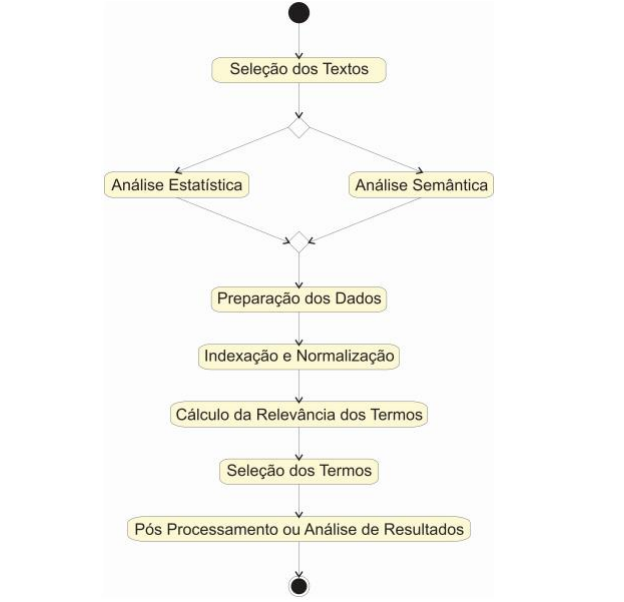
\includegraphics[scale=0.8]{figuras/figura_2.PNG} % altere o atributo scale para o tamanho da figura
	\end{center}
	\legend{Fonte: \cite{morais2007mineraccao}}
\end{figure}

\subsubsection{Abordagem dos dados}
\cite{morais2007mineraccao} apresenta dois tipos de abordagem dos dados textuais na área de mineração de textos: Análise Semântica, baseada na funcionalidade dos termos encontrados no texto, e Análise Estatística, baseada na frequência dos termos encontrados no texto. Estas abordagens podem ser utilizadas de forma separada ou em conjunto. A abordagem utilizada neste trabalho é a Análise Semântica.

\subsubsubsection{Análise Semântica}
Análise que avalia a sequência dos termos no texto sendo analisado, para identificar sua função, fundamentada em técnicas de \textit{Processamento de Linguagem Natural}. A análise semântica se dá pelo pelo conhecimento do significado das palavras de forma individual, independente do contexto, e também pelo conhecimento da estrutura dessas palavras, por exemplo, ao determinar os limites da palavra que determinam seu radical. A utilização de Análise Semântica se dá pela melhoria na qualidade dos resultados do processo de mineração de textos \cite{morais2007mineraccao}. 

Como as técnicas de análise semântica de textos procuram identificar a importância das palavras dentro da estrutura de orações \cite{morais2007mineraccao}, e por estar diretamente relacionada ao \textit{processamento de linguagem natural}, esse conceito é utilizado neste trabalho durante o pré-processamento dos dados, detalhado no Capítulo 5.


\subsubsection{Preparação dos dados}
A preparação dos dados envolve a seleção de dados que constituem a base de textos de interesse e o trabalho inicial para tentar selecionar o núcleo que melhor expressa o conteúdo desses textos. Além de prover uma redução dimensional, esta etapa procura identificar similaridades em função da morfologia ou do significado dos termos nos textos. O primeiro passo do processo de prepação dos dados é a \textit{Recuperação de Informação} \cite{morais2007mineraccao}. Um \textit{Sistema de Recuperação de Informação Textual} é um sistema desenvolvido para indexar e recuperar documentos do tipo textual. Nesse tipo de sistema as consultas são descritas através de termos e os documentos relevantes são recuperados de acordo com esses termos.

Outra etapa da preparação dos dados é a Análise de Relevância, onde o usuário pode entrar com um termo e obter como resposta um resultado de um problema em particular. A Análise de Relevância é utilizada principalmente para filtrar dados não pertencentes ao conjunto obtido. Essa etapa não é realizada, tendo em vista que os comentários coletados já compõem a base de dados desejada.

O ytCommentMiner \footnote{https://github.com/ssisaias/ytCommentMiner}, software desenvolvido para coleta dos comentários, é responsável pela etapa de preparação dos dados, até o momento da coleta dos textos online. A ferramenta não implementa a etapa de Análise de Relevância sobre o conjunto obtido.

\subsubsection{Indexação e Normalização}
O objetivo principal da indexação e normalização dos textos é facilitar a identificação de similaridade de significado entre suas palavras, considerando variações morfológicas e problemas de sinonímia \cite{morais2007mineraccao}. Este processo tem como resultado a geração de um índice, construído através de um processo de indexação. Um documento pode ser indexado por termos diferentes que são correspondentes ao vocabulário utilizado em sua área. Nesse caso, geralmente, há um conjunto de termos predefinidos e específicos para cada assunto da área em questão \cite{morais2007mineraccao}.

Em mineração de textos, a indexação é um processo automático. Suas principais fases são: \textit{identificação de termos} (simples ou composto); remoção de \textit{stopwords} (palavras irrelevantes); e \textit{normalização morfológica} (stemming) \cite{morais2007mineraccao}.

\begin{figure}[H] %use h para forçar que a figura fique abaixo do texto
	\caption{\label{fig:figura-4} Etapas do Processo de Indexação Automática}
	\begin{center}
	    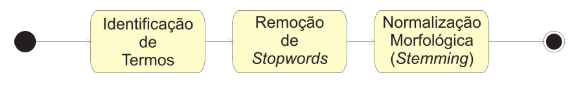
\includegraphics[scale=0.8]{figuras/figura_4.PNG} % altere o atributo scale para o tamanho da figura
	\end{center}
	\legend{Fonte: \cite{morais2007mineraccao}}
\end{figure}

A identificação dos termos consiste em identificar os termos contidos nos textos, sejam palavras simples ou termos compostos por duas ou mais palavras, também pode ser realizada uma correção dos erros gramaticais atravé de um dicionário de termos \cite{morais2007mineraccao}. 

Remoção de \textit{stopwords} consiste em eliminar palavras que não devem ser consideradas no documento, conhecidas como \textit{stopwords}. \textit{Stopwords} são palavras não relevantes ao texto, por não traduzirem sua essência. Normalmente fazem parte da lista de \textit{stopwords} preposições, pronomes, artigos, advérbios e outras classes de palavras auxiliares \cite{morais2007mineraccao}.

Também durante o processo de indexação, torna-se interessante remover as variações morfológicas de uma palavra, através da identificação do seu radical. Os prefixos e os sufixos são removidos, e apenas o radical resultante é adicionado ao índice. Essa técnica é chamada de lematização ou \textit{stemming} \cite{morais2007mineraccao}.

A identificação dos termos, remoção dos stopwords e \textit{steeming}, neste trabalho são realizados automaticamente através de \textit{scripts} e descritos no Capítulo 5.

\subsubsection{Cálculo de relevância dos termos}
Com exceção das \textit{stopwords}, os termos mais frequentemente utilizados no texto, costumam ter maior importância, assim como palavras constantes em títulos ou em outras estruturas, uma vez que foram colocadas ali por serem consideradas relevantes para a idéia do documento \cite{morais2007mineraccao}.

O cálculo de relevância de uma palavra em relação ao texto que está inserida pode se basear na frequência da mesma, na análise estrutural do documento, ou na posição sintática da palavra. Ao grau de relacionamento da palavra com o texto dá-se o nome de \textit{peso}. Logo é o peso que indica a importância da palavra em relação ao texto \cite{morais2007mineraccao}. 

\cite{morais2007mineraccao} apresenta algumas formas para cáculo do peso, que utilizam cálculos simples de frequência: \textit{frequência absoluta}, \textit{frequência relativa}, \textit{frequência inversa de documentos}. Nenhuma dessa técnicas é utilizada neste trabalho. Neste trabalho, o cálculo da relevância dos termos é realizado ao preparar o dicionário da ferramenta \textit{Sentistrength}, onde é possível dar um nível de relevância para cada palavra individualmente.

\subsubsection{Seleção dos termos}
Seleção de termos corresponde à etapa de seleção das palavras retiradas do texto, após os
processos de pré-processamento e cálculo da relevância. Esta técnica pode ser baseada no peso dos termos ou na sua posição sintática em relação ao texto. Entre as principais técnicas de seleção dos termos está a \textit{Seleção por análise de linguagem natural} \cite{morais2007mineraccao}, utilizada neste trabalho.

\subsubsubsection{Seleção por análise linguagem natural}
A \textit{seleção por análise de linguagem natural} consistem em aplicar técnicas de análise sintática ou semântica para identificar palavras em um documento. A análise semântica baseia-se no princípio de que as partes mais relevantes de um documento já estão de alguma forma demarcadas por estruturas de formatação específicas para isso \cite{morais2007mineraccao}.

A \textit{Seleção por análise de linguagem natural} é utilizada pelo autor tanto no momento da extração dos textos dos conjuntos de comentários obtidos, como durante a montagem do modelo de classificação, tendo em vista que há uma classificação prévia do grupo de treino dos comentários e uma triagem dos comentários classificados antes de serem utilizados para criação de fato do modelo.

\subsubsection{Pós processamento ou análise dos resultados}
Esta fase envolve a aplicação de técnicas de análise dos resultados de um Sistema de Recuperação de Informações de Texto, particularmente os resultados do processo de mineração de textos. A análise pode ser utilizada como forma de avaliação do \textit{Sistema de Recuperações de Informação de Texto}, para saber se funcionou como deveria ou não \cite{morais2007mineraccao}.

Entre as principais métricas de análise de \textit{Sistema de Recuperações de Informação de Texto} estão: \textit{recall} e \textit{precision}.

\subsubsubsection{\textit{Recall}}
O \textit{recall} (abrangência ou revocação) mede a habilidade do sistema em recuperar os documentos mais relevantes para seu usuário, com base no termo ou expressão utilizado na formulação de sua busca \cite{morais2007mineraccao}.

Sua fórmula consiste em:

\begin{equation}
\label{eq:recall-description-morais}
 {recall} = \frac{{n-recuperados-relevantes}}{{n-possiveis-relevantes}}, onde:
\end{equation}

n-recuperados-relevantes: é o número de documentos relevantes recuperados.

n-possíveis-relevantes: é o número total de documentos relevantes do sistema. Essa informação
geralmente não é conhecida e só pode ser estimada estatisticamente.

\subsubsubsection{\textit{Precision}}
A \textit{precision} (precisão) mede a habilidade do sistema em manter os documentos irrelevantes fora do resultado de uma consulta \cite{morais2007mineraccao}.

Sua fórmula consiste em:

\begin{equation}
\label{eq:precision-description-morais}
 {precision} = \frac{{n-recuperados-relevantes}}{{n-total-recuperados}}, onde:
\end{equation}

n-recuperados-relevantes: é o número de documentos relevantes recuperados.

n-total-recuperados: é o número total de documentos do sistema.


\subsection{Processamento de Linguagem Natural}
\cite{liddy2001naturallanguage} define \textit{Processamento de Linguagem Natural (Natural Language Processing - NLP)} como um conjunto de técnicas para analisar e representar textos de origem natural, em um ou mais níveis de análise linguística com o propósito de atingir processamento linguístico similar ao humano para um conjunto de tarefas ou aplicações. 

Para mineração de textos armazenados em formato não estruturados, são necessárias técnicas e ferramentas específicas da área de \textit{Descoberta de Conhecimento em Textos (Knowledge Discovery from Text - KDT)} \cite{morais2007mineraccao}. Para recuperação de informação, KDT e mineração de textos possuem alto grau de dependência de Processamento de Linguagem Natural.
% Na Seção, processamento em linguagem natural explicar a técnica NLP. Detalhar como ela é utilizada.
Neste trabalho, NLP é utilizada tendo em vista que o ato de interpretar e manipular palavras como parte de uma linguagem é considerado Processamento de Linguagem Natural \cite{morais2007mineraccao}.


\subsection{SentiStrength}
SentiStrength é um classificador léxico que utiliza regras de linguística para detectar a força de um sentimento em uma frase \cite{thelwall2012sentistrength}.

Para cada texto classificado, a ferramenta gera dois valores inteiros que variam de 1 a 5 numa escala positiva e 1 a 5 numa escala negativa, sendo o valor 1, um indicador de neutralidade para o sentimento. Por exemplo, uma classificação que retorna 3, 5 indica uma nota 3 para o sentimento positivo e nota 5 para o sentimento negativo, nesse caso o texto tem mais força negativa do que positiva \cite{thelwall2012sentistrength}.

O classificador SentiStrength foi concebido para ser utilizado com diversos idiomas, porém seu dicionário padrão é em inglês. É possível adaptar seu dicionário para outros idiomas. O dicionário utilizado pelo autor neste trabalho, parte de um dicionário português limitado que é fornecido no site da ferramenta SentiStrength, porém adaptado com mais palavrões e algumas correções, para uma detecção mais abrangente. A lista completa dos palavrões adicionados, assim como sua relevância na classificação é indicada no Apêndice B. O dicionário utilizado, em sua completude, pode ser encontrado no Apêndice A. Além disso, foi feito um script \footnote{https://gist.github.com/ssisaias/08b2c8494a4553612987c9d4ae94f86c} para converter a classificação gerada pela ferramenta, para a entrada esperada pelo classificador Naïve Bayes, essa etapa é descrita na seção de procedimentos.


\subsection{Naive Bayes}
Segundo \cite{tan2009DataMining}, uma técnica de classificação é uma maneira de construir modelos de classificação a partir de um \textit{Dataset}. Exemplos de classificadores são: Árvore de decisão; Rede Neurais; SVM (Support Vector Machines); e classificadores Naïve Bayes.
Cada uma dessas técnicas aplica um algoritmo de aprendizagem para identificar o modelo que melhor descreve um relacionamento entre o conjunto de atributos e as classes dos dados de entrada. Sendo assim o modelo gerado pelo algoritmo de aprendizagem deve ser capaz de, a partir de um conjunto de entradas, classificar corretamente registros que não eram conhecidos até então.

Naïve Bayes é um dos algoritmos mais eficientes para \textit{machine learning} e mineração de textos. Esse algoritmo de aprendizagem supervisionado utiliza do Teorema de Bayes, porém considerando haver independência entre as \textit{features} (característica das variáveis de entrada) do conteúdo sendo classificado \cite{zhang2004optimalitybayes}.

De acordo com com \cite{zhang2004optimalitybayes}, o Teorema de Bayes com \textit{features} dependentes pode ser definido da seguinte maneira, onde por exemplo, a probabilidade $P$ de um $comentario$ ser de classe $c$ é:

\begin{equation}
\label{eq:bayes_classic}
 P(c|comentário) = P(c) \frac{P(comentario |c)}{P(comentario)}
\end{equation}

Considerando existem duas classes, \textbf{positivo} e \textbf{negativo}, o evento $comentario$ pertence a classe $positivo$ se somente se:

\begin{equation}
\label{eq:bayes_classic}
 {f_b}(comentario) =  \frac{P(positivo| comentario)}{P(negativo| comentario)} \geq 1
 
\end{equation}

onde ${f_b}(comentario)$ é um classificador Bayesiano.

Ao assumir que as \textit{features} são independentes dados os valores de classe, ou seja:

\begin{equation}
\label{eq:naive_bayes}
 {p}(comentario|c) =  {p}({comentario_1, comentario_2, ..., comentario_n}|c) = \prod_{i=1}^{n} {p}(comentario_i|c),
\end{equation}

O classificador resultante é:

\begin{equation}
\label{eq:bayes_classic}
 {f_nb}(comentario) =  \frac{P(positivo)}{P(negativo)} \prod_{i=1}^{n} \frac{P({comentario_i} | positivo)}{P({comentario_i} | negativo)}
\end{equation}

A função ${f_nb}(comentario)$ é chamada de classificador Naive Bayes (Naïve Bayesian Classifier).


Neste trabalho é utilizada uma instância de Naïve Bayes chamada \textit{Multinomial Naïve Bayes}. \textit{Multinomial Naïve Bayes} indica que ${p}(comentario_i|c)$ possui uma distribuição multinomial. \textit{Multinomial Naïve Bayes} é altamente recomendado para processamento de texto não estruturado onde há contagem de palavras ao considerar a relevância dos termos \cite{metsis2006whichnaivebayes}.
A criação de um modelo Multinomial Naïve Bayes se dá através da ferramenta \textit{scikit-learn}, onde o processo de criação do classificador já é previamente implementado. \textit{scikit-learn} é uma biblioteca de aprendizagem de máquina desenvolvida na linguagem \textit{Python} \cite{scikit-learn}. 



\newpage
\section{TRABALHOS RELACIONADOS}

%Trabalhos de mineração de textos (Lucas, Priscila, morais e ambrósio)
Explorar comentários de vídeos do Youtube é uma área de pesquisa recente e ainda em crescimento. Os trabalhos de \citeonline{ammari2011filteringYt} e \citeonline{schultes2013leave} são pesquisas relativamente recentes que possuem coleta, mineração e classificação desses comentários.

O trabalho de \citeonline{ammari2011filteringYt} faz parte de um grupo maior de pesquisas, que visam elaborar um modelo de usuário que possa ser utilizado em simuladores de aprendizagem. Seu foco é apresentar uma técnica de filtragem de comentários com baixo valor semântico para o domínio selecionado, coletados de mídias sociais. A técnica proposta combina aprendizagem de máquina, mineração de dados, e análise semântica, a fim de obter comentários que sejam relevantes para o domínio desejado. A construção do modelo foi feita utilizando os classificadores Naïve Bayes Multinomial e Árvore de Decisão C4.5.

\citeonline{ammari2011filteringYt} coletou 1159 comentários de 17 vídeos do Youtube, dos quais 5 vídeos tiveram 193 comentários selecionados para o grupo de controle do modelo. A técnica apresentada e utilizada por \citeonline{ammari2011filteringYt} é mostrada na Figura \ref{fig:ammari-metodologia}:

\begin{figure}[H] %use h para forçar que a figura fique abaixo do texto
	\caption{\label{fig:ammari-metodologia} Metodologia de filtragem para comentários de baixo valor semântico do Youtube.}
	\begin{center}
	    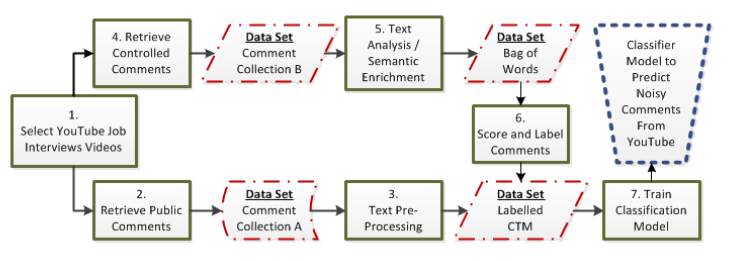
\includegraphics[scale=0.8]{figuras/figura_3.PNG} % altere o atributo scale para o tamanho da figura
	\end{center}
	\legend{Fonte: \citeonline{ammari2011filteringYt}}
\end{figure}

A metodologia da Figura \ref{fig:ammari-metodologia} consiste em:

\textbf{1.} Selecionar vídeos sobre entrevistas de emprego no Youtube.

\textbf{2.} Coletar os comentários públicos dos vídeos selecionados.

\textbf{3.} Pré-Processar os comentários obtidos.

\textbf{4.} Selecionar um grupo de comentários para grupo de controle, esses comentários são considerados relevantes para o domínio de entrevistas de emprego selecionado.

\textbf{5.} Analisar os comentários do grupo de controle, a fim de obter um Corpo de Palavras enriquecido semanticamente, relevante para o domínio.

\textbf{6.} Pontuar os comentários para facilitar sua classificação, que no caso do trabalho \cite{ammari2011filteringYt} é \textit{relevant} (relevante) ou \textit{noisy} (ruidoso - com baixo valor semântico).

\textbf{7.} Com os comentários devidamente pontuados, treinar um modelo de classificação supervisionado que irá indicar se um comentário é relevante ou não para o domínio proposto.

Os resultados apresentados por \cite{ammari2011filteringYt} indicam um alta taxa de acerto dos classificadores para os comentários obtidos e pré-processados com a metodologia proposta, sendo 86,7\% de corretude para o algoritmo C4.5 e 83,7\% para o Naïve Bayes Multinomial.

A principal diferença entre \cite{ammari2011filteringYt} e este trabalho é que apesar de focar inicialmente em vídeos com público infantil e adolescente, este trabalho é capaz de aplicar o modelo em qualquer grupo de comentários de vídeos do Youtube. Dessa forma, expandindo o domínio de aplicação. Considerando também que modelo de \cite{ammari2011filteringYt} foi testado com 17 vídeos da plataforma porém um total de 1159 comentários, este trabalho avaliou um total de 87.094 comentários pertencentes a canais difundidos entre jovens e crianças, como \textbf{Galinha Pintadinha} e \textbf{Felipe Neto}.


\citeonline{schultes2013leave} afirmam em seu texto que comentários em vídeos do Youtube são, de forma geral, mal vistos pelo público: em uma pesquisa com 95 participantes, 64\% consideram comentários do Youtube "irrelevantes", 42\% consideram agressivos e 51\% os consideram "estúpidos", sendo que somente 6\% dos entrevistados consideram os comentários em vídeos do Youtube "De essencial importância". Por outro lado, \citeonline{schultes2013leave} também afirma que 34\% dos entrevistados leem os comentários dos vídeos e que 53\% lê os primeiros três comentários antes de começar a assistir o vídeo, além de estimar um total de 96 milhões de autores de comentários ativos na plataforma, chegando a conclusão de que a seção de comentários em vídeos do Youtube é uma funcionalidade essencial e uma das mais usadas em vídeos online. Levando esses fatores antagônicos em consideração, \cite{schultes2013leave} primeiramente procura verificar se comentários em vídeos do Youtube geram algum valor agregado e como medir esse valor. \cite{schultes2013leave} também prova que através dos comentários é também possível obter uma análise semântica do vídeo em questão. 

No período de 15/03/2012 à 21/03/2012, \cite{schultes2013leave} coletou um total de 136.854 comentário dentre 304 vídeos do Youtube de categorias variadas. Para tentar descobrir se os comentários agregam algum valor para o leitor, foi proposto agregá-los em três tipos de comentários:
\begin{itemize}
    \item \textbf{Discussão:} Comentários que geram debates dentre os usuários da plataforma;
    \item \textbf{Comentários inferiores:} Comentários com ofensas ou conteúdo irrelevante para o vídeo em questão; 
   \item \textbf{Comentários substanciais:} Comentários não ofensivos que contém informação relevante e estão relacionados com o tema do vídeo em questão.
\end{itemize}
Após definir os tipos de comentários, ainda foram definidos dez subtipos a fim de tornar a classificação mais concisa. % Esses 10 tipos foram omitidos a fim de manter a brevidade desse texto.
Durante a validação do seu \textit{Dataset}, \citeonline{schultes2013leave} concluiram que "não existe um tipo de comentário dominante em vídeos do Youtube"\ e também que "30\% dos comentários são do tipo \textbf{Comentários inferiores}\", o que pode explicar a má impressão dos usuários em relação aos comentários em vídeos do Youtube.

Apesar de ter utilizado um grupo maior de comentários do que este trabalho, \citeonline{schultes2013leave}, os vídeos obtidos são de diversas categorias tornando o modelo gerado menos específico.

%Mario falcao
Sobre proteção de crianças online, \citeonline{marioFalcao2016} aborda em sua pesquisa o problema da falta de acompanhamento por parte dos pais, quanto a utilização da internet por seus filhos. 

\cite{marioFalcao2016} propos um sistema multiagente composto por agentes que coletaram e analisaram dados do Facebook. Os agentes trabalham juntos para trazer dados relevantes para o modelo de classificação, que auxilia em detectar casos de aliciamento infantil. O algoritmo utilizado para a classificação foi de árvore de decisão J48 \cite{quinlan1986induction}, implementado no WEKA, uma ferramenta de mineração de dados gratuita. O modelo foi validado com o perfil do Facebook de duas crianças, com o consentimento dos pais, e os resultados foram satisfatórios onde o modelo mostrou que uma das crianças apresentava-se em grupo de risco e estaria possivelmente sendo aliciada por adultos. 
Em comparação, o foco deste trabalho não é detectar possíveis aliciadores, mas sim determinar se a seção de comentários de um vídeo de Youtube é seguro para a criança que está assistindo o vídeo, sendo uma outra camada de proteção para as crianças. O trabalho \cite{marioFalcao2016} também chegou a verificar a eficácia do seu modelo com outros algoritmos de classificação, entre eles o Naive Bayes que é utilizado neste trabalho.

%EnyoGonçalves
\cite{EnyoGoncalves2017} estende o trabalho de \cite{marioFalcao2016}, buscando detectar automaticamente quando uma mensagem suspeita é trocada entre uma criança e um adulto. O algoritmo de classificação utilizado é Naive Bayes Multinomial \cite{metsis2006spamBayes}.

Os dados utilizados para treinar o modelo com mensagens "perigosas"\ foram coletados do site: \footnote{http://www.perverted-justice.com}. Os dados com mensagens consideradas "normais"\  foram retirados do site: \footnote{http://vircio.net}. Foram utilizadas 1610 mensagens ao todo, com um total de 9450 palavras, para as quais o Naive Bayes Multinomial obteve uma taxa de acerto de 86,33\%. Após aplicar o modelo em conversa real entre uma criança e um suspeito de aliciamento, \cite{EnyoGoncalves2017} mostrou que seu modelo é mais robusto que o de \cite{marioFalcao2016}, pois pode detectar frases de aliciadores fora de contexto e além disso, detecta frases como um todo e não somente palavras-chave.

A tabela, a seguir, apresenta uma comparação entres os trabalhos citados anteriormente e este trabalho em questão:


\begin{table}[H]
	\Caption{\label{tabela-trabalhos} Comparação entre trabalhos relacionados e este trabalho}%
	{%
		\begin{tabular}{p{4cm}p{5cm}p{6cm}} %{p{3cm}ccp{4.5cm}} não fica maior que o texto, horizontalmente
			\toprule
			Trabalho & Tipo de Aplicação &  Objetivo \\
			\midrule \midrule
    		\cite{ammari2011filteringYt} & Minerar comentários do Youtube & Filtrar comentários do Youtube com pouco valor semântico.\\
    		\hline	
			\cite{schultes2013leave} & Minerar comentários do Youtube & Verificar a relevância de comentários do Youtube.\\
			\hline
			\cite{marioFalcao2016} & Proteção de crianças online & Medir nível de exposição de crianças no Facebook.\\
			\hline
			\cite{EnyoGoncalves2017} & Proteção de crianças online & Detectar facilmente aliciadores de crianças na internet.\\
			\hline
			Este trabalho & Mineração de comentários do Youtube e proteção de crianças online & Verificar se um comentário de vídeo do Youtube é adequado ou não para crianças.\\
			\bottomrule
		\end{tabular}%
	}{%
	\Fonte{Elaborado pelo autor}
}
\end{table}


\begin{comment}
\textcolor{red}{Duas observações sobre essa tabela de comparação de trabalhos relacionados: \\
1. Prefira não deixar as colunas com valores binários. Ao invés de a coluna proteção de crianças, colocar tipo de aplicação. E como valor ao invés de sim e não descrever qual tipo de aplicação que pode ser proteção da criança.\\ <- Concluido
2. Por mais que você tenha colocado aqui as diferenças e semelhancas entre o seu trabalho e os relacionados, é necessário você descrever essa semelhanças e diferenças em algum paragrafo.} <- Checando
\end{comment}

\newpage
\section{PROCEDIMENTOS METODOLÓGICOS}

Para alcançar o objetivo de classificar os comentários pejorativos em vídeos infantis do Youtube, os passos a seguir descritos na Figura \ref{fig:metodologia} foram planejados. A execução dos passos é descrita no Capítulo 6.


\begin{figure}[H] %use h para forçar que a figura fique abaixo do texto
	\caption{\label{fig:metodologia} Ilustração do procedimento metodológico}
	\begin{center}
	    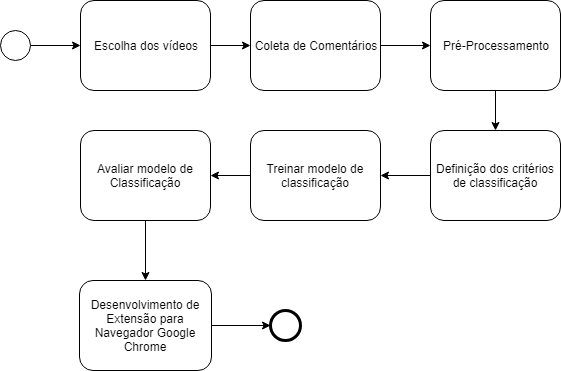
\includegraphics[scale=0.7]{figuras/figura_6.png} % altere o atributo scale para o tamanho da figura
	\end{center}
	\legend{Fonte: autor}
%Verificar se precisa por a data aqui 
\end{figure}


% Mudar o tempo para futuro
\subsection{Escolha dos vídeos}
O principal critério para a escolha do vídeo para este trabalho, é que seu público alvo seja infantil ou adolescente. Naturalmente, quanto mais comentários o vídeo possuir, maior a quantidade de dados para análise, logo o ideal é buscar vídeos infantis que apresentam um número expressivo de comentários, em torno de pelo menos mil. Porém, tendo em consideração que nem sempre é possível encontrar vídeos com essa quantidade ideal de comentários, podem ser utilizados vídeos com menos comentários. A popularidade dos canais que postaram os vídeos é um fator a ser considerado, visto que um canal com maior popularidade, tende a possuir vídeos com mais comentários.


\subsection{Coleta de Dados}
A fim de ter os dados para o ponto de partida da pesquisa e tendo em conta a grande quantidade de comentários em vídeos com público-alvo jovem, foi desenvolvida uma ferramenta em Python para coleta dos comentários em vídeos do Youtube. O objetivo da ferramenta é ser simples e objetiva na coleta desses comentários. A ferramenta é responsável pela etapa de preparação dos dados, dentro dos conceitos de mineração de texto.


\subsection{Pré-Processamento}
Uma vez que os dados armazenados não estão em formato adequado para extração do conhecimento, faz-se necessária a aplicação de métodos para \textit{extração, integração,} \textit{transformação},
% ta mas o que é isso? ai vou precisar olhar no referencial teórico e adaptar conforme o que eu fiz aqui!!!
\textit{limpeza}, \textit{seleção e redução} de volume desses dados, antes da etapa de mineração \cite{morais2007mineraccao}.

Inicialmente, observa-se uma grande quantidade de comentários sem sentido em vídeos infantis no Youtube, compostos quase que inteiramente por espaços em branco ou símbolos e letras aleatórios. Em vídeos destinados à adolescentes, há menor ocorrência de comentários sem sentido. 

Faz necessário a utilização de um método ou ferramenta que fará a limpeza dos textos, bem como a aplicação da ferramenta NLTK para que seja feito o pré-processamento dos textos. Um \textit{script} foi criado pelo autor e sua utilização é detalhada no Capítulo 6.


\subsection{Definição dos Critérios de Classificação}

A classificação dos comentários é definida manualmente, levando em consideração comentários de amostragem, que serão classificados como \textbf{pejorativos} ou \textbf{não pejorativos}. 

Dado a enorme quantidade de comentários coletados, um dicionário de classificação também será criado para a ferramenta \textbf{SentiStrength}, a fim de facilitar a criação do conjunto de treino a ser dado de entrada para gerar o modelo de classificação. 

Após a classificação manual e a classificação assistida utilizando a \textit{SentiStrength}, um modelo deve ser construído a partir do treinamento  com o conjunto de dados coletados, para que se  possa classificar automaticamente os novos comentários obtidos do Youtube.

\subsection{Treinamento do Modelo de Classificação}
O classificador Naïve Bayes recebe um conjunto de dados de treino, e um conjunto de testes para averiguar a precisão do modelo de classificação \cite{ZhangandLi2007Bayes}. Esses conjuntos de dados são escolhidos de forma aleatória dentre os comentários obtidos.

Por meio da ferramenta \textit{Sentistrength}, pode-se obter um grupo de comentários classificados automaticamente, que deve ser analisado e melhorado pelo autor, a fim de obter um modelo de classificação mais preciso.

\subsection{Definição dos critérios de classificação}
A definição dos critérios de classificação corresponde à avaliação do modelo de classificação, ou seja, da sua qualidade.
O modelo gerado poderá ser testado, utilizando os comentários que não foram utilizados na fase de treino, ou seja, utilizando os comentários selecionados para compor o conjunto de teste. 

A avaliação do modelo é feita através da ferramenta \textit{Scikit-learn}, que fornece métodos de \textit{score} prontos para as medidas de \textit{precision} e \textit{recall}.



\subsection{Desenvolvimento de Extensão para Navegador Google Chrome}

Por meio do desenvolvimento de um \textit{plugin} para o Google Chrome é possível utilizar o modelo construído e indicar vídeos com comentários pejorativos.
Nessa etapa, são avaliados os resultados do processamento dos comentários, agregando agora pelos vídeos dos quais foram coletados, indicando quais os vídeos tem maiores taxas de comentários pejorativos e que não são considerados seguros para crianças e adolescentes.



\newpage
\section{AVALIAÇÃO EXPERIMENTAL}


Para elaboração do modelo de classificação, a partir dos comentários obtidos para o vídeo \textbf{Não Faz Sentido! - Crepúsculo [+13]}, foram escolhidos de forma aletória um grupo de 50\% (32.131) dos comentários para elaboração do modelo de classificação e 50\% (32.130) dos comentários para elaboração do grupo de validação (ou grupo de testes).
Neste Capítulo é descrita toda a execução dos passos mencionados na Figura \ref{fig:metodologia} e no Capítulo 5, utilizando os grupos de comentários para elaboração e validação do modelo.
% Passos sugeridos de acordo com os objetivos específicos:
% Classificar os comentários: (1) Coleta de Dados (2) Pré-Processamento (3) Definição dos Critérios de Classificação
% Analisar os comentários: (4) Treinamento do Modelo de Classificação
% Indicar os vídeos Pejorativos (5) xxxxxx
% Avaliar o modelo de classificação (6) Avaliação do Modelo de Classificação
\subsection{Escolha dos vídeos}
Levando em consideração os critérios de escolha mencionados anteriormente, o tamanho do canal que postou o vídeo e a quantidade de comentários, foram escolhidos os vídeos a seguir:

\begin{itemize}  
    \item \textbf{PARABÉNS DA GALINHA PINTADINHA - Clipe Música Oficial - Galinha Pintadinha DVD 4} \footnote{https://www.youtube.com/watch?v=ei2-RjJDBHc}
	\item \textbf{Galinha Pintadinha 4 - Clipe Música Oficial - Galinha Pintadinha DVD 4} \footnote{https://www.youtube.com/watch?v=gWI4qV2H8VY} 
	\item \textbf{UPA CAVALINHO - Clipe Música Oficial - Galinha Pintadinha DVD 4} \footnote{https://www.youtube.com/watch?v=Fn9adh4HWUU}
	\item \textbf{Pintinho Amarelinho - DVD Galinha Pintadinha} \footnote{https://www.youtube.com/watch?v=59GM\_xjPhco} 
	\item \textbf{Galinha Pintadinha 3 - Trailer - OFICIAL} \footnote{https://www.youtube.com/watch?v=FTC-MEUmZLw}
	\item \textbf{Não Faz Sentido! - Crepúsculo [+13]} \footnote{https://www.youtube.com/watch?v=2Lp7XO6oWCM} 
\end{itemize}


\subsection{Coleta de Dados}
Para coletar os comentários dos vídeos, uma aplicação na linguagem \textit{Python} foi desenvolvida pelo autor. O Software ytCommentMiner \footnote{https://github.com/ssisaias/ytCommentMiner} utiliza a API do Youtube (Versão 3) e permite tanto obter os comentários de topo (\textit{top level comments} ou \textit{Comment Threads}), como as réplicas à esses comentários, dado o ID do vídeo que pode ser encontrado na sua URL, permitindo obter todos os comentários públicos disponíveis no vídeo, até o momento da coleta.

Os comentários são armazenados na máquina onde ytCommentMiner está sendo executado no formato de dados JSON, contendo meta informações relacionadas aos comentários: ID do comentário, nome do autor, texto original da postagem, texto atual da postagem, data de publicação e total de réplicas. A Figura \ref{fig:comentario_coletado} mostra um comentário coletado pela ferramenta em formato JSON, o nome do autor do comentário foi omitido.

\begin{figure}[H] %use h para forçar que a figura fique abaixo do texto
	\caption{\label{fig:comentario_coletado} Exemplo de comentário obtido pela ferramenta ytCommentMiner}
	\begin{center}
	    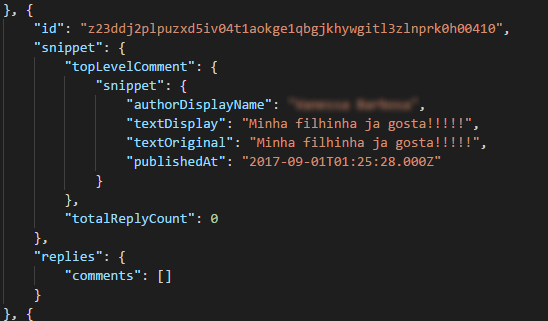
\includegraphics[scale=1]{figuras/figura_comentario_coletado.png} % altere o atributo scale para o tamanho da figura
	\end{center}
	\legend{Fonte: autor}
%Verificar se precisa por a data aqui 
\end{figure}


\subsection{Pré-Processamento}

Nesta etapa, um \textit{script} \footnote{https://gist.github.com/ssisaias/d6dd83361d6fa64c0341427b1f6f3f22} escrito em Python foi executado para extrair somente os textos dos comentários obtidos através da ferramenta de extração, o script também é capaz de remover caracteres que não são considerados, dentro do contexto desta pesquisa, como \textit{emojis}. 

Em seguida, através da ferramenta NLTK, o pré-processamento foi realizado de foram automática: os acentos foram removidos e os textos foram \textit{tokenizados}, através de um processo que remove palavras sem valor semântico para o classificador e reduz palavras com valor semântico ao seu radical, através dos métodos \textit{word\_tokenize()} e \textit{RSLPStemmer()} presentes na NTLK. Ao final dessa etapa, um arquivo contendo os comentários devidamente pré-processados é gerado. 

\subsection{Treinamento do Modelo de Classificação}
Em posse dos comentários pré-processados, foi obtido um modelo de classificação da seguinte forma:

Primeiramente, o dicionário da \textit{SentiStrength} deve estar previamente estabelecido, o autor obteve um dicionário pronto para a língua portuguesa já fornecido no site da ferramenta e o melhorou e adaptou para o contexto deste trabalho, removendo algumas palavras em inglês que estavam erroneamente no dicionário e adicionando os palavrões necessários para a classificação de comentários com termos pejorativos. Os palavrões adicionados podem ser encontrados no Apêndice B.

A versão do \textit{SentiStrength} utilizada foi a 2.3, específica para Sistemas Operacionais Windows. Através de sua interface gráfica, o arquivo foi gerado pelo \textit{script} \footnote{https://gist.github.com/ssisaias/d6dd83361d6fa64c0341427b1f6f3f22} da etapa de pré-processamento. Após a classificação gerada pelo \textit{SentiStrength}, alguns comentários foram verificados manualmente pelo autor, esse procedimento se refere à classificação assistida. Frases que foram classificadas como pejorativas erroneamente por possuírem, por exemplo, o seguinte \textit{emoticon} \textbf{:(}, foram reclassificadas como neutras, pelo próprio autor. Ou seja, não expressão sentimento pejorativo.

Outro \textit{script}\footnote{https://gist.github.com/ssisaias/08b2c8494a4553612987c9d4ae94f86c} é então executado para "\textbf{traduzir}" a classificação feita pela \textit{SentiStrength}. O funcionamento desse \textit{script} se dá do seguinte modo: Quando a classificação de um comentário é dada como positiva pela ferramenta, é então convertida para \textbf{0} (ou classificação neutra); Quando a classificação é negativa, espera-se que haja um termo pejorativo no comentário e esse é classificado com o valor \textbf{1}. Isso faz com que o modelo de classificação apenas se preocupe com as duas classes determinadas que são neutra e pejorativa.

De posse dos comentários que compõem o grupo de treino devidamente classificados, utilizou-se a biblioteca \textit{scikit-learn}, para criação do modelo de classificação. O procedimento está descrito a seguir. 

No trecho de código abaixo, as variáveis \textbf{counts} e \textbf{targets} representam a lista com os comentários e a lista com suas classificações, respectivamente. A variável \textbf{classifier} recebe a nova instância do classificador MultinomialNB, e que em seguida é "alimentada"\ com os dados dos comentários e sua classificação. O modelo de classificação é então criado.

\begin{lstlisting}[frame=single, language=Python]  % Start your code-block

from sklearn.naive_bayes import MultinomialNB 
classifier = MultinomialNB()
classifier.fit(counts,targets)

\end{lstlisting}


\subsection{Avaliação do Modelo de Classificação}

Nesta etapa, os comentários separados para o grupo de teste foram submetidos ao classificador. Também foram submetidos todos os outros comentários obtidos, tendo estes passado pelo mesmo procedimento de pré-processamento, classificação na ferramenta \textit{SentiStrength}, análise humana, e enfim, classificados pelo modelo gerado anteriormente.

A exemplo do grupo de testes mencionado na criação do modelo de classificação, uma matriz com os comentários é passada para o método \textbf{predict()} do classificador. A variável \textbf{predictions} contém a classificação gerada, que agora pode ser avaliada de acordo com os valores esperados.

\begin{lstlisting}[frame=single, language=Python]  
predictions = classifier.predict(teste_counts)
\end{lstlisting}

A avaliação do modelo é feita através da ferramenta Scikit Learn, que fornece métodos de \textit{score} prontos para as medidas de \textit{precision} e \textit{recall}. Um \textit{script} \footnote{https://gist.github.com/ssisaias/b9521c910d66c440c9e90d21f5360536} auxiliar foi criado com os passos de validação. Os resultados da avaliação são apresentados no próximo capítulo.



\subsection{Extensão do Google Chrome - SafeYoutube}

Após gerar e avaliar o modelo de classificação, e obter os resultados, foi desenvolvida uma extensão do navegador da web Google Chrome que se utiliza de um \textit{Web Service} que retorna a margem de comentários negativos e positivos para o vídeo sendo assistido naquele momento.

A extensão \textbf{SafeYoutube} foi criada utilizando as tecnologias web HTML, CSS e Javascript. Como referência para o desenvolvimento foi utilizada a documentação oficial para desenvolvedores Chrome \footnote{https://developer.chrome.com/extensions}. Sua arquitetura é descrita no diagrama da Figura \ref{fig:chrome_plugin_design}. Os códigos-fonte da extensão \footnote{https://github.com/ssisaias/safe-youtube} e do serviço web \footnote{https://github.com/ssisaias/safe-youtube-service}, estão disponíveis publicamente e podem ser encontrados na plataforma Github.

\begin{figure}[H] %use h para forçar que a figura fique abaixo do texto
	\caption{\label{fig:chrome_plugin_design} Arquitetura da extensão desenvolvida}
	\begin{center}
	    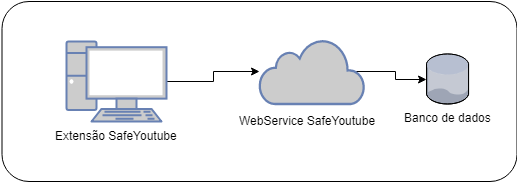
\includegraphics[scale=0.7]{figuras/safeYoutube.png} % altere o atributo scale para o tamanho da figura
	\end{center}
	\legend{Fonte: Autor}
%Verificar se precisa por a data aqui 
\end{figure}

Ao entrar um vídeo do youtube com a extensão \textbf{SafeYoutube} instalada, ela permite que o usuário a selecione, exibindo assim os resultados de uma classificação realizada previamente para aquele vídeo. Um exemplo do funcionamento é visto na Figura \ref{fig:chrome_plugin}. 

Caso os comentários do vídeo ainda não tenham sido classificados, o serviço irá iniciar um procedimento automático de classificação, tornando os resultados disponíveis dentro de um intervalo de tempo. O procedimento automático de classificação segue os mesmo procedimentos listados nas etapas de \textbf{pré-processamento} e \textbf{avaliação do modelo}, ou seja, os comentários são coletados, pré-processados, e classificados com o modelo de classificação gerado na etapa de \textbf{Treinamento do Modelo}.

\begin{figure}[H] %use h para forçar que a figura fique abaixo do texto
	\caption{\label{fig:chrome_plugin} Extensão SafeYoutube}
	\begin{center}
	    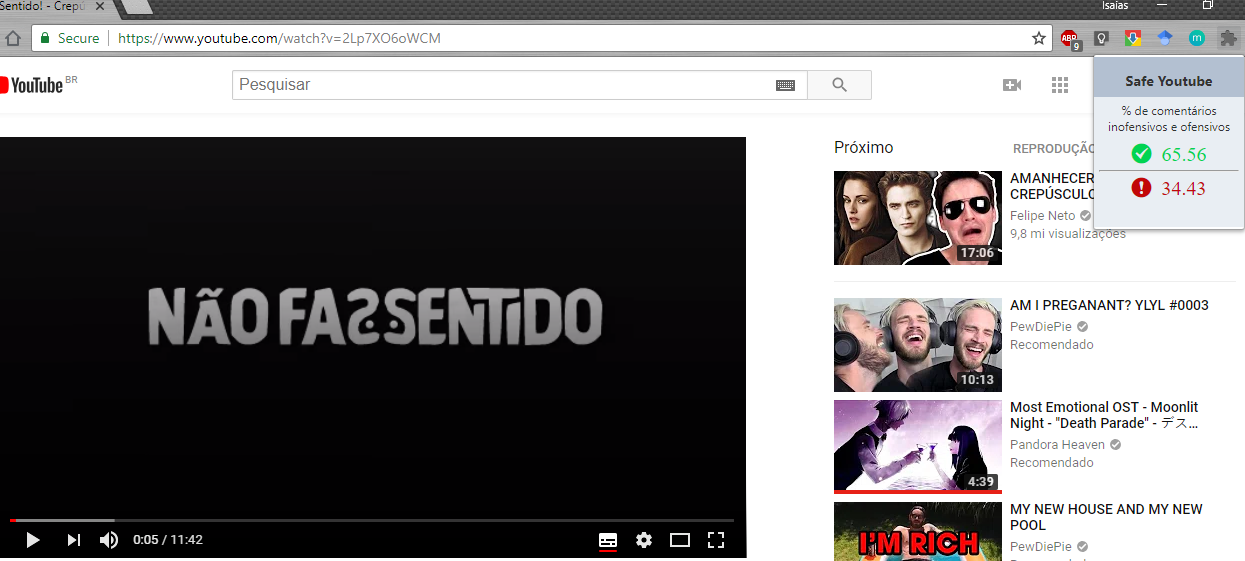
\includegraphics[scale=0.4]{figuras/extensao_chrome_normal.png} % altere o atributo scale para o tamanho da figura
	\end{center}
	\legend{Fonte: Autor}
%Verificar se precisa por a data aqui 
\end{figure}

\begin{figure}[H] %use h para forçar que a figura fique abaixo do texto
	\caption{\label{fig:chrome_plugin_zoom} Extensão SafeYoutube - Imagem ampliada}
	\begin{center}
	    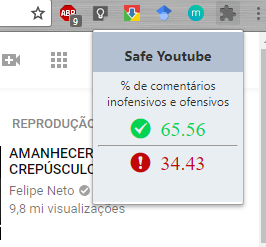
\includegraphics[scale=0.7]{figuras/extensao_chrome_zoom.png} % altere o atributo scale para o tamanho da figura
	\end{center}
	\legend{Fonte: Autor}
%Verificar se precisa por a data aqui 
\end{figure}

Nota-se pelo \textit{plugin} no canto superior direito da Figura \ref{fig:chrome_plugin_zoom}, que o vídeo em questão possui 65.56\% de comentários positivos e 34.43\% de comentários negativos.



\newpage
\section{RESULTADOS}

Foram coletados 87.094 comentários ao todo, dentre 5 vídeos infantis e 1 vídeo com público adolescente.
A Tabela \ref{resultados-pre-comentarios} apresenta os meta dados da base adquirida: nome dos vídeos,  total de visualizações no momento da coleta, data da coleta e quantidade de comentários por vídeo.

\begin{table}[H] \footnotesize
\centering
	\Caption{\label{resultados-pre-comentarios} Vídeos selecionados e comentários obtidos}%
%META-DADOS	
\begin{tabular}{|p{5.5cm}|c|c|c|}
\hline
\textbf{Título do Vídeo} & \textbf{Visualizações} & \textbf{Data da Coleta} & \textbf{Comentários obtidos} \\ \hline
PARABÉNS DA GALINHA PINTADINHA - Clipe Música Oficial - Galinha Pintadinha DVD 4 & 388.515.807 & 20/11/2017 12:00 & 11.669 \\ \hline
Galinha Pintadinha 4 - Clipe Música Oficial - Galinha Pintadinha DVD 4 & 90.240.721 & 20/11/2017 11:30 & 2.320 \\ \hline
UPA CAVALINHO - Clipe Música Oficial - Galinha Pintadinha DVD 4 & 112.389.836 & 27/09/2017 23:38 & 2.798 \\ \hline
Pintinho Amarelinho - DVD Galinha Pintadinha & 496.289.054 & 28/09/2017 00:05 & 12.906 \\ \hline
Galinha Pintadinha 3 - Trailer - OFICIAL & 13.849.870 & 27/09/2017 11:28 & 298 \\ \hline
Não Faz Sentido! - Crepúsculo [+13] & 15.768.111 & 15/05/2018 07:14 & 57.103 \\ \hline
% MEU MELHOR AMIGO - LUCCAS NETO & 14.762.043 & 11/06/2018 02:21 & 46.173 \\ \hline
\end{tabular}

\Fonte{Elaborado pelo autor}
\end{table}

Por conta do vídeo \textbf{Não Faz Sentido! - Crepúsculo [+13]} ser o com maior quantidade de comentários e devido ao seu público alvo ser composto por adolescentes, o conjunto de treino e de testes da classificação partiu dele. 

% Tabela 3
A Tabela \ref{resultados-qtd-commentarios-classes} exibe a quantidade de comentários obtidos em cada classe, para cada vídeo analisado. Esse total é obtido através do método \textit{classification\_report()} presente na biblioteca \textit{scikit-learn}.

\begin{table}[H] \footnotesize
\centering
	\Caption{\label{resultados-qtd-commentarios-classes} Quantidade de comentários em cada classe por vídeo}%
%Comentarios positivos x negativos	
\begin{tabular}{|p{5.5cm}|c|c|}
\hline
\textbf{Título do Vídeo} & \textbf{Neutros} & \textbf{Pejorativos} \\ \hline
PARABÉNS DA GALINHA PINTADINHA - Clipe Música Oficial - Galinha Pintadinha DVD 4 & 11.152 & 517 \\ \hline
Galinha Pintadinha 4 - Clipe Música Oficial - Galinha Pintadinha DVD 4 & 2.217 & 103 \\ \hline
UPA CAVALINHO - Clipe Música Oficial - Galinha Pintadinha DVD 4 & 2.654 & 144 \\ \hline
Pintinho Amarelinho - DVD Galinha Pintadinha & 11.407 & 1.499 \\ \hline
Galinha Pintadinha 3 - Trailer - OFICIAL & 277 & 21 \\ \hline
Não Faz Sentido! - Crepúsculo [+13] & 21.066 & 11.064 \\ \hline

\end{tabular}

\Fonte{Elaborado pelo autor}
\end{table}

Como foi descrito no Capítulo 6, o modelo gerado foi utilizado em todos os comentários obtidos, com exceção dos comentários utilizados no grupo de treino, tendo sido a etapa de geração do modelo de classificação, o único passo a ser executado somente uma vez. Além disso, apesar do grupo a partir do qual foi gerado o modelo de classificação ter partido de apenas um vídeo, os comentários negativos são similares dentre todos os vídeos, seja de conteúdo infantil ou juvenil.
\begin{comment}
\textcolor{red}{Não entendi Isaias, como você calculou recall e precision dos comentários dos outros projetos, se você não os avaliou com a SentiStregth... ou avaliou? Isso não fica claro e gera algumas dúvidas. Além disso, é bom dizer que mesmo que você tenha usado somente de um tipo de video, os comentários para criar o modelo e o testar, você tem comentários similares nos outros vídeos...}
\textcolor{pink}{I: Todos foram avaliados com Sentistrength, vou deixar mais explicito aqui e também na metodologia. Sobre os comentários similares, irei mencionar.}
\end{comment}
Seguindo a metodologia de 50\% de comentários para treino e 50\% para teste do classificador, foram utilizados 32.131 comentários para treino e 32.130 comentários para teste. 

Em relação à analise de dados com conjuntos de dados de entrada desbalanceados, para um modelo de classificicação, \cite{tan2009DataMining} afirma que as métricas de \textbf{\textit{precision}} e \textbf{\textit{recall}} se sobressaem à métrica de \textit{taxa de acertos}, pois esta última não considera o peso das classes sendo analisadas.

Na Tabela \ref{resultados-precision} estão os valores de \textit{precision}, descritos por vídeo, após a classificação. Os valores são obtidos com o uso da biblioteca \textit{sklearn-metrics} \cite{scikit-learn}. A coluna \textbf{precision-pos} descreve a precisão de acerto do classificador para a classe positiva (ou neutra), enquanto a coluna \textbf{precision-neg} descreve a precisão de acerto do classficador para a classe negativa, onde estão os termos pejorativos.

Na Tabela \ref{resultados-recall} estão os valores de \textit{recall}, também descritos por vídeo e classe. A coluna \textbf{recall-pos} descreve a pontuação de \textit{recall} para a classe de comentários positivos (ou neutra), enquanto a coluna \textbf{recall-neg} descreve a pontuação de recall para a classe de comentários pejotarivos.


%\textcolor{red}{Chamar de negativo de pejorativo parece pouco intuitivo. Uma vez que desejamos saber se um vídeo contem comentários pejorativos ou não. O que você acha?} - I: Sim, me convenceu;


%\textit{Precision} pode ser definido como o número de (eventos) Positivos-Verdadeiros dividido pela soma entre Positivos-Verdadeiros e Positivos-Negativos (ou seja,aqueles que foram classificados como negativo 

Nas definições a seguir, $T_p$ (\textit{True positive} ou positivo verdadeiro) indica o número de comentários da classe de comentários positivos (neutros) que foram corretamente detectados como positivos; $F_n$ (\textit{False negative} ou falso negativo) denota a quantidade de comentários pejorativos detectados erroneamente como positivos; $F_p$ (\textit{False positive} ou falso positivo) indica a quantidade de comentários pejorativos detectados erroneamente como positivos; e $T_n$ (\textit{True negative} ou negativo verdadeiro) indica a quantidade de comentários pejorativos detectados corretamente \cite{tan2009DataMining}.

\textit{Precision} pode ser definida para a classe de comentários positivos, por exemplo, como a proporção do número de acertos pelo modelo na classe positiva pelo número de instâncias que foram classificadas como positiva pelo modelo. 

%\textcolor{red}{Por favor, explique melhor o que é $T_P$ e $F_P$, pode até buscar no livro do Tan} <- Buscando. <- Done

\begin{equation}
\label{eq:precision-descr}
 {P} = \frac{{T_p}}{{T_p}+{F_p}}
\end{equation}


Enquanto o \textit{recall}, corresponde a proporção do número de acertos, por exemplo, da classe positiva divido pelo que é realmente positivo.

\begin{equation}
\label{eq:recall-descr}
 {R} = \frac{{T_p}}{{T_p}+{F_n}}
\end{equation}

\begin{table}[H] \footnotesize
\centering
	\Caption{\label{resultados-precision} Resultados de \textit{precision}}%
	
\begin{tabular}{|p{5.5cm}|c|c|c|}
\hline
\textbf{Título do Vídeo} & \textbf{Classificados} & \textbf{precision-pos} & \textbf{precision-neg} \\ \hline
PARABÉNS DA GALINHA PINTADINHA - Clipe Música Oficial - Galinha Pintadinha DVD 4 & 11.669 & 0.98 & 0.18 \\ \hline
Galinha Pintadinha 4 - Clipe Música Oficial - Galinha Pintadinha DVD 4 & 2.320 & 0.98 & 0.14 \\ \hline
UPA CAVALINHO - Clipe Música Oficial - Galinha Pintadinha DVD 4 & 2.798 & 0.98 & 0.16 \\ \hline
Pintinho Amarelinho - DVD Galinha Pintadinha & 12.906 & 0.95 & 0.35 \\ \hline
Galinha Pintadinha 3 - Trailer - OFICIAL & 298 & 0.95 & 0.14 \\ \hline
Não Faz Sentido! - Crepúsculo [+13] & 31.130 & 0.88 & 0.71\\ \hline
\end{tabular}

\Fonte{Elaborado pelo autor}
\end{table}

\begin{table}[H] \footnotesize
\centering
	\Caption{\label{resultados-recall} Resultados de \textit{recall}}%
	
\begin{tabular}{|p{5.5cm}|c|c|c|}
\hline
\textbf{Título do Vídeo} & \textbf{Classificados} & \textbf{recall-pos} & \textbf{recall-neg} \\ \hline
PARABÉNS DA GALINHA PINTADINHA - Clipe Música Oficial - Galinha Pintadinha DVD 4 & 11.669 & 0.86 & 0.71 \\ \hline
Galinha Pintadinha 4 - Clipe Música Oficial - Galinha Pintadinha DVD 4 & 2.320 & 0.84 & 0.57 \\ \hline
UPA CAVALINHO - Clipe Música Oficial - Galinha Pintadinha DVD 4 & 2.798 & 0.81 & 0.64 \\ \hline
Pintinho Amarelinho - DVD Galinha Pintadinha & 12.906 & 0.83 & 0.67 \\ \hline
Galinha Pintadinha 3 - Trailer - OFICIAL & 298 & 0.78 & 0.48 \\ \hline
Não Faz Sentido! - Crepúsculo [+13] & 31.130 & 0.83 & 0.79\\ \hline
\end{tabular}

\Fonte{Elaborado pelo autor}
\end{table}

A partir dos resultados apresentados nota-se que o classificador possui uma alta taxa de \textit{precision} para a classe positiva, enquanto apresenta taxas menores para a classe de comentários pejorativos, onde se encontram os termos pejorativos.

Essa diferença se dá principalmente pela quantidade de comentários negativos detectados e presentes, pois pode-se notar na Tabela \ref{resultados-qtd-commentarios-classes}, vídeos com público alvo infantil possuem menor quantidade de comentários negativos detectados.

Por outro lado, a pontuação de \textit{recall} para comentários negativos foi satisfatória para 4 dos 6 vídeos analisados, mostrando que dentre os comentários pejorativos de fato existentes, o classificador gerado conseguiu detectar corretamente sua maior parte. Novamente, é possível notar que as menores taxas de \textit{recall} se dão nos vídeos com menos comentários e com menor quantidade de comentários negativos, vide Tabela \ref{resultados-qtd-commentarios-classes}.


\newpage
\section{CONCLUSÃO}

% \textcolor{red}{utilize os verbos em terceira pessoa do singular ou do plural, nunca em primeira pessoa.}  <- Corrigindo

A partir dos resultados apresentados nota-se que o classificador possui uma alta taxa de \textit{precision} para a classe positiva, enquanto apresenta taxas menores para a classe de comentários pejorativos, onde se encontram os termos pejorativos.

Essa diferença se dá principalmente pela quantidade de comentários negativos detectados e presentes, pois se pode ver na tabela \ref{resultados-qtd-commentarios-classes}, vídeos com público alvo infantil possuem menor quantidade de comentários negativos detectados.

Por outro lado, a pontuação de \textit{recall} para comentários negativos foi satisfatória para 4 dos 6 vídeos analisados, mostrando que dentre os comentários pejorativos de fato existentes, o classificador gerado conseguiu detectar corretamente sua maior parte. Novamente é possível notar que as menores taxas de \textit{recall} se dão nos vídeos com menos comentários e com menor quantidade de comentários negativos, vide Tabela \ref{resultados-qtd-commentarios-classes}.%criar tabela.

% não sei se posso falar algo do tipo: vídeos infantis tem menor taxa de comentários ofensivos enquanto que vídeos com público adolescente tem maior taxa de comentários ofensivos.

Logo nota-se que quanto mais comentários o vídeo apresentar, maior a taxa de acerto eventos de comentários negativos e maior a relevância da classificação realizada.
Os dados obtidos podem ser de fato considerados úteis para a classificação de comentários pejorativos de vídeos no Youtube, mais precisamente vídeos com público alvo adolescente. O que torna relevante o uso da extensão criada para o navegador da web Google Chrome.


% ----------------------------------------------------------
% ELEMENTOS PÓS-TEXTUAIS
% ----------------------------------------------------------
%\postextual

% Referências bibliográficas

\renewcommand{\refname}{REFERÊNCIAS}
\begingroup
\raggedright
\bibliography{bibtex/referencias}
\endgroup
\addcontentsline{toc}{section}{REFERÊNCIAS}
      
% Glossário (Consulte o manual da classe abntex2 para orientações sobre o glossário)
%\glossary

% Apêndices
\apendice{APÊNDICE A}
\addcontentsline{toc}{section}{APÊNDICE A}

% DICIONÁRIO UTILIZADO NA FERRRAMENTA SENTISTRENGTH


\begin{longtable}{|*3{p{15cm}|}}
\caption{Dicionário Utilizado na Ferramenta Sentistrength} \label{appendix:dicionario-sentistrength}
    \hline
ADVERS, AGU, ALOL, AOK, Admir, Admoni, Agraciados, Apaixonado, Apesar, Avaric, Blur, Cuidado, Céu, DAMAG, DIN, ECSTA, EXIGÍVEL, Excel, Faixas, Feroc, Festiv, Fiel, Fuckface, Graci, Grati, Harmon, Honesto, InVigor, Joll, Lazie, Lucki, Mar, Moody, Muah, Nast, PRIVILEG, Pettie, RAID, Romântico, SAP, Shaki, Splend, Tortur, Tosspot, TrEMBL, Treacher, UGL, Virtuo, abafado, abandonar, abate, abatido, abdicar, abençoar, aberração, abertura, abestado, abismo, abjeto, abolir, abominar, abominável, aborrecer, aborrecido, aborrecimento, abrasivo, abraço, abraços, abrupto, absurdo, abusi, abuso, abutre, acalentar, acaso, accus, acidente, acossado, acostar, acrimon, acrobacia, acusação, adepto, adjudicação, adoecer, ador, adora, adoração, adoro, adorável, adulterar, adulterat, adultério, adventur, adversário, afetação, afeto, afiado, afligir, aflição, afogar, afundou, agarrar, aggravat, agitado, agitar, agitat, agitação, agonia, agoniz, agradeceu, agradável, agredir, agreeab, ai, alarme, alegar, alegação, alegrar, alegremente, alegria, aleijado, alienat, almejar, altercação, altivo, alívio, ama, amado, amante, amarfanhar, amargo, amarrotar, amavelmente, amaz, ambiguit, ambivalente, ambíguo, ameaça, amor, amoroso, amputar, amus, analfabeto, anarquia, anarquista, anexo, angr, angústia, animosidade, aniquilar, aniquilação, anomalia, anormais, ansiar, ansioso, antagoni, anti-social, antieconômico, antinatural, antipatia, antiquado, antitrust, anular, anulação, anus, anxi, anômalo, apagar, aparência, apath, aplicar, apoio, aposentar, appreciat, apprehens, apreciar, apreender, apressado, aprisionar, apuro, apóia, arbitrário, ardente, argh, argumentos, arma, armadilha, arraste, arrebatar, arrepio, arriscado, arrogan, arrogante, arruda, arsehole, arteiro, artificial, asham, asinino, assaltar, assalto, assassinato, assassino, assinalada, assombrar, assustador, assustando, asswipe, astuto, ataque, atarantado, atencioso, aterroriza, aterrorizado, aterrorizar, atordoa, atrair, atrasado, atraso, atrofia, atroz, aturdido, ausente, austero, ausência, autocrata, autocrático, avaliado, avarento, aversi, aviltar, azarado, azedo, açougue, baba, baba-ovo, babaca, babaca, babaovo, baboseira, bacura, bagos, bagunça, bagunçado, baitinga, baitola, baixa, baixar, bala, balbuciar, banal, banana, bandido, banir, baque, baranga, baranga, barato, barbari, barf, barreira, barulho, bastardo, batalha, bater, batida, beaut, bebum, bebê, bebês, beicinho, beijo, beijoca, beligerante, beligerantes, bem, berk, berrante, besta, besta, bestial, bff, bg, bicha, bicha, birdbrain, bisbilhotar, bisca, biscate, bixa, bizarro, blah, blam, blefando, blefe, bloco, blurt, boa, bobagem, bobagens, bobo, bocejo, boceta, boco, bocó, boiola, bolagato, bom, bomba, bondade, bonehead, bonito, boquete, bosseta, bosta, bostas, brandir, brando, bravata, breve, briga, brilho, brillian, brincadeira, brincalhão, brincando, brioco, brocha, bronha, broxa, brusco, bruta, brutal, bruto, bruxa, bruxaria, buceta, buceta, bufão, bug, bulir, bullshit, \\ bumhole, bunda, bunduda, burgl, burlista, burro, burro, busseta, bélico, bêbado, bônus, cachorra, cadela, cadela, caga, cagado, cagao, cagona, cagão, calamidade, calandra, calma, calmaria, calmarias, calúnia, canalha, canalha, cancelar, canhão, canibal, cansado, cansativo, cansaço, caos, capitular, capotar, caprichoso, captura, cara de pau, caralho, carenagem, carga, carinho, carniça, caro, carranca, carrancudo, carrossel, casseta, cassete, cataclismo, catástrofe, cauteloso, cavalo, caverna, caçador, caótico, ceder, cegos, censor, censura, cercear, cerco, cerda, chafurdar, chama, chamuscar, chantagem, charlatanismo, charlatao, charlatão, chata, chateado, chatice, chato, chato, cheio, chereca, chicote, chifruda, chifrudo, chochota, choque, chora, choradeira, choramingar, chorando, chorar, chorou, chota, chuckl, chupada, chupado, chupar, chás, cicatriz, cinzento, ciumento, clamor, claro, coaxar, cobiçar, cocaina, cocaína, cocksucker, coercitivo, colapso, colidir, colisão, combate, combatente, comed, comemorar, cometer, comiseração, como, comoção, compaixão, companheiro, compartilhada, compartilhar, compelir, competir, complicar, complicação, compulsão, comum, cona, concurso, condenar, condenação, condescen, confiante, confiança, confinar, confiscar, confisco, confissão, conflito, conforto, confrontar, confundir, confus, confusão, congestionado, congestionamento, conluio, conspirador, conspirar, conspiração, consternação, constranger, contagioso, contenda, contentamento, contente, contorcer, contorcer-se, contra, contrabandear,  contradições, contrariar, controvers, contrário, contusão, convencido, cool, corna, corno, corroer, corrosivo, corrosão, corrupto, corrupção, cortar, corte, courag, covarde, coxo, craZ, crap, crappy, crasso, crepitar, cretina, cretino, crime, crise, critici, cruel, cruz, crye, crédulo, crítica, crítico, crônica, cu, cuidados, cuidar, culpa, culpado, culpável, cumplicidade, curalho, cuzao, cuzuda, cuzudo, cuzão, câncer, cãibra, cético, cínico, cú, dEspis, danado, danos, debil, debiloide, decadente, decadência, decapitar, declínio, decompos, defeito, defenc, defensiva, deficiente, deficiência, definhar, defunto, degenerar, degradantes, deitado, delectabl, delgado, delicioso, delicious, deligh, delinquente, delinquência, delírio, demissão, demitido, demitir, demitir-se, demolir, demonio, demônio, demônio, denegrir, dente, denunciar, dependentes, deplorar, deplorável, depor, depravado, depreciar, depreciativo, depreciação, deprimir, derramar, derrota, derrubada, derrubar, desabilitar, desacostumado, desacreditar, desafiador, desafiar, desafio, desagradável, desajeitado, desajustamento, desalojar, desamparado, desanima, desanimador, desanimar, desanimei, desaparecer, desapontar, desarmar, desastre, desastroso, descarado, desconcertado, desconfiança, desconforto, desconhecido, desconsiderar, descontentamento, descontrole, descortês, descrença, descuidado, desculpe, desdém, desempenhado, desempregados, desenraizar, \\ deserto, deserção, desespero, desfavoráveis, desfazer, desfeito, desfigurado, desfiladeiro, desgosto, desgracado, desgracados, desgraça, desgraçado, desgraçado, desgraçados, desgrenhado, desigual, desigualdade, desilusão, desinformados, desinteresse, desistente, desisti, desleal, desleixado, deslocar, deslumbrante, desmaiar, desmentir, desmoralizar, desmoronar, desnecessária, desobediente, desobediência, desolado, desolador, desolação, desonesto, desonra, desordem, desorganizado, desorientar, despejar, desperat, despercebido, despertaram, despesa, despreocupado, desprezo, desprezível, desproporcionada, desprotegido, desprovido, destemido, destruct, destruir, desumano, desvantagem, desvantajoso, desviar, desvio, desânimo, deter, determinado, determinação, detestar, deturpar, devastadores, devastar, devastação, deve, devedor, devot, diabo, diabólico, dickhead, difamar, difamação, diferem, dificuldade, difunto, difícil, digni, dilema, dilúvio, diminuir, diminuição, dinâmi, direito, disagre, disapprov, discordante, discrepante, discriminar, discriminação, discutível, discórdia, disfarce, disparar, disparate, dispendioso, dispensabilidade, dispensar, dispor, disputa, disputável, dissatisf, dissidência, dissimulado, dissipar, dissolução, dissuadir, distanciamento, distrair, ditar, ditatorial, divagar, divertido, divin, divisão, divórcio, diâmetro, doce, docemente, doces, doente, doentes, doentio, doença, doida, doido, dominar, dominação, dor, dores, dork, douchebag, downhearted, doçura, duvidoso, débil, défice, dúvida, easie, eejit, egotis, egoísta, ei, elegan, eliminar, eliminação, elogio, emaranhar, embaraçar, emboscada, emocional, emoção, empe, empinar, empt, empurrão, empurrões, encanto, encargos, encoberto, encontrão, encorajando, enemie, energ, enervar, enferrujado, enfurecer, enga, enganador, enganando, enganar, enganação, engano, enganosa, enganoso, engolfar, enjôo, enlouquecedora, enrag, enrijecer, enrolação, enrolão, ensolarado, enterrada, enterrar, enthus, entorpecido, entorse, entravar, entupir, envergonhado, envie, epidemia, epíteto, equívoco, erosão, erradicar, errado, errar, erro, errôneo, esbanjar, esboçado, escaldadura, escandaloso, escape, escaramuça, escassez, escasso, esconder-se, escoriáceo, escravidão, escravizar, escrota, escroto, escrutinar, escurecer, escuro, escárnio, escândalo, escória, esfregaço, esgotar, esgoto, esgueirar-se, esmagado, esmagador, esmagar, esnobe, esotérico, espancado, espancar, especial, espera, esperado, esperando, esperança, esperançosamente, esperançoso, espinhoso, esporrada, esporrado, esporro, espreitar, espástico, esquecimento, esquisitice, estafado, estagnado, estelionatario, estelionato, estelionatário, estigma, estola, estragar, estranged, estrangeiro, estrangeiros, estrangulamento, estrangular, estranho, estremecimento, estresse, estridente, estrita, estupida, estupidez, estupido, estupor, estuprador, estuprando, estupro, estáticas, estéril, estúpida, estúpido, estúpido, evasão, evitar, exagerando, exasperat, excedente, excentricidade, excessiva, excesso, excluir, exclusão, excommunicat, excremento, excruciat, \\ excêntrico, executar, execuções, expediente, expelir, explodir, explosiva, explosão, expor, exprobrar, expulsar, exterminat, extinguir, extinto, extravagante, extraviados, extraviar-se, exílio, fab, fabricat, fabuloso, faca, facada, facilidade, facilmente, fake, falecimento, falha, falhado, falido, fallout, falsear, falsidade, falsificação, falso, falta, falácia, famintos, fantástico, fanático, faroleiro, farrapo, farsa, fascinação, fascista, fastidioso, fatal, fathead, fatigu, favor, fdp, febre, febril, fedelho, feder, fedida, fedido, fedor, fedor, fedorenta, feia, feio, feiosa, feioso, feioza, feiozo, fel, fela, felacao, felação, feliz, ferida, ferido, ferimento, ferir, feroz, fervilhar, festa, feudo, fiança, fiasco, fiesta, filho da puta, fingir, fiofó, fiscal, flagrante, flertar, flexib, flexibilização, foda, foda-se, fodao, fode, foder, fodida, fodido, fodido, fodão, fofoca, fome, forgiv, forjado, formidável, fornica, forte, força, fraco, fratura, fraude, fraude, frenético, fricção, frio, frustrante, frustrar, frágeis, frígido, frívolo, fucker, fucks, fuckwit, fuctard, fud, fude, fudecao, fudendo, fudeção, fudida, fudido, fuga, fugaz, fugir, fugitivo, fugiu, fugly, fulera, fuleragem, fumaça, fuming, fundador, funn, furioso, furnica, furnicar, futilidade, fácil, fé, fúria, fútil, gaguejar, galo, ganhou, ganido, ganância, garança, garra, gaseado, gasto, gay, geek, gemer, gemido, genero, gentlest, germe, gibberi, giggl, glori, glória, gmbo, golpe, golpeado, golpista, gonorrea, gonorreia, gordura, gosta, gostei, gosto, gracioso, grande, gratef, gratuito, grave, graves, gravidade, graxos, graça, graças, grelinho, grelo, greve, griev, grinn, gritar, grosseiro, grotesco, grr, guerra, guerras, guerreado, guerrilha, gueto, guincho, h8, ha, habitar, haha, handsom, happi, hater, heartbroke, heartwarm, hediondo, hehe, herói, hesita, hijack, hilário, hipocondríaco, hipocrisia, hipócrita, histeria, histérico, hogwash, hoho, homossexual, honra, hooey, horda, horr, horrorizado, horrível, hostil, hugg, humilhante, humor, hungr, hurra, ideal, idiota, idiotas, idiotice, ignor, ignóbil, ilegal, ilegalidade, iludir, ilusão, ilógico, imaturo, imbecil, imobilidade, imoral, impasse, impatien, impedimento, impedir, imperfeito, impessoal, impetuoso, impiedoso, implacável, implicar, implorar, impopular, impor, importan, impotente, imprecisão, impressionar, imprevistas, imprudente, impróprio, impulsivo, impureza, impuro, imundo, imóveis, imóvel, inacessível, inacreditável, inadequa, incapacidade, incapaz, incentivo, incerto, incessante, incivil, inclinação, incoerências, incomodar, incompatib, incompeten, inconstante, inconvenien, incorreta, incrível, incurável, incómodo, indecente, indecis, independentemente, indesejáveis, indetermin, indeterminado, indevido, indiferente, indiferença, indigente, indignação, indigno, indisciplinado, indisposição, indizível, ineffect, ineficiência, inesperadamente, inevitável, inexatidão, inexato, inexperiente, inexplicável, infame, infantil, infectar, infecção, infeliz, infelizmente, inferior, infernal, inferno, inferno, infestar, infiel, infiltração, inflamado, inflamar, inflação, infligir, infortúnio, infracção, \\ infração, infrutífero, ingratidão, ingrato, ingénuo, inimigo, injunção, injustificada, injusto, innocen, inofensivo, inquietante, inquieto, insalubre, insano, insatisfatória, insecur, insegurança, inseguro, insensível, insidioso, insignificante, insincer, insinuar, insolente, insolência, inspir, instabilidade, instável, insufficien, insulto, insuportável, inteligente, intell, intempestivo, interferência, interrupção, intimidar, intimidat, intolerante, intolerável, intoxicar, intrometer-se, intrometido, intrud, intrusão, inundar, invadir, inveja, invejoso, invisível, involuntário, inválido, inábil, inépcia, inútil, ira, ironia, irracional, irrefletido, irregular, irresponsável, irrisório, irritar, irritação, irritável, irônico, isca, iscrota, iscroto, isentar, isola, jerked, jittery, jogar, jurar, juros, jurou, kenga, kindn, labuta, ladra, ladrao, ladroeira, ladrona, ladrão, ladrão, laidback, lalau, lamacento, lamentar, lamentação, lamento, lança, lapso, laço, legal, lento, leprosa, leproso, lesma, ligeira, likeab, limitação, linguado, liquidar, liquidação, litig, livel, livrar, livrará, lixo, lmao, lodo, lol, lolol, lorota, loucamente, louco, loucura, lous, loveless, lucked, lucks, lucro, ludibriacao, ludibriar, ludibriação, lunkhead, lunático, luta, lutado, lutar, luv, lágrima, lágrimas, machorra, machucar, macumba, maddest, magnific, mal, mal-estar, malandragem, malandro, malcriado, maldito, maldição, malicioso, maligno, maltratar, maluquinho, malícia, mancada, mancar, mancha, mandriar, manguaca, manguaça, manhoso, mania, manipulat, mano, manso, maníaco, maravilha, maravilhosa, maravilhoso, marginal, masmorra, masochis, massacre, masturba, matador, matar, meanie, medo, medonho, medos, medíocre, melanchol, melancolia, melhor, melhorar, melodramático, mendigar, mendigo, mentira, mentiras, mentiroso, mentiu, merda, merda, merdoso, meretriz, merr, mija, mijada, mijado, mijo, mijo, minado, minar, miserável, misses, mistak, misunderst, mocrea, mocreia, mocréa, mocréia, mogoloid, moleca, moleque, molestar, monotonia, monstro, monstruoso, monótono, morrer, mortal, mortalha, morte, mortif, mortos, mourejar, mudo, muito, muleke, muleque, multa, multicor, mundano, murchar, murmurar, musaranho, muthafuck, mácula, mártir, mérito, míope, namorada, narcótico, naufrágio, nazista, nebulosidade, nebuloso, necessitado, negado, negar, negativo, negação, negligen, negligenciar, negligente, negligência, nerd, nervoso, neurótico, neutralizar, neutralização, ninhada, nix, nojeira, nojenta, nojento, nojo, nonsens, notório, novato, ntre, nucklehead, numpty, nurtur, nutter, não, obcecar, obes, obliterar, oblíquo, obnóxio, obrigada, obrigado, obscurecer, obsoletos, obstinado, obstruir, obstrução, obstáculo, ociosidade, oco, ocultar, odeia, odeio, odiando, odiava, odio, odioso, ofender, ofensa, offens, ok, okays, oks, omfg, omg, omissão, omitir, openminded, opor, oposição, opportun, oprimir, optimi, orgulho, orgulhoso, original, otaria, otario, otarios, otária, otário, otários, ousadia, outrag, padrão, painf, paining, painl, paixão, palatabl, palhaçada, pandemônio, \\ panelinha, parafuso, paralisadas, paralisados, paralisação, paralisia, paranoi, parar, parasita, paraíso, partes, partie, partilha, partição, parto, paspalha, paspalhao, paspalho, paspalhão, pateta, patetice, patife, patético, pau, pavor, paz, pecado, pecados, pecaminoso, peculiar, peido, pena, penal, pendurar, penis, pensativo, pequenino, pequeno, perambular, perda, perde, perdedor, perder, perdida, perdido, perdição, perdoou, perecer, perereca, perfeito, perigo, perigosas, perigosos, perplexidade, persecut, perseguição, perturbado, perturbar, perverso, perversão, pesadelo, pesado, pesar, pessimis, petrif, petulância, phobi, piada, pica, picada, picao, picão, pilantra, pilantragem, pillock, pinhead, pior, piranha, piroca, piroco, piru, pisar, pistoleiros, pitada, piti, pleasur, plebeu, plonker, pneu, pobres, pobreza, podre, podridão, poluentes, pomposo, pontapé, popa, populares, porra, porra, porte, positiv, pqp, praga, prais, prannock, prat, precioso, precipitado, precário, predicamento, prega, preguiça, preguiçosamente, preguiçoso, prejudic, prejudica, prejudicado, prejudicando, prejudicar, prejudiciais, prejudicial, preocupação, presidiário, pressentimento, pressur, presunçoso, presunção, pretensioso, pretensão, prettie, prisão, problema, procrastinar, procrastinação, prod, proibir, promis, prontidão, pronto, propaganda, prostituta, protelando, protesto, provação, provocar, provocação, prêmio, puk, punheta, punhetao, punhetão, punho, punir, puro, pus, puta, putaria, puto, puxa-saco, puxasaco, pária, pânico, pênis, quebrou, queda, queimar, queixar-se, queixoso, quenga, quentes, querida, querido, questionável, quitação, rabao, rabo, rabuda, rabudao, rabudo, rabudona, rabudão, rabão, racha, rachadinha, racis, radiano, radical, raiva, ralhar, ralo, rampante, rancor, rançoso, rapariga, raptar, rasgar, raso, raspar, rastejar, rato, ração, reacionário, reassur, reativa, rebelde, recalcitrante, recaída, recessão, recompensa, recorrida, recuo, recusa, recusar, redundan, refrão, refugiados, refutar, regozijar, regresso, rejeitar, relaxar, reluctan, relutante, remorso, renunciar, renúncia, repartição, repreensão, repreensível, reprimir, reprovação, repudiar, repugnante, repulsa, repulsivo, resistente, resmungar, resmungão, resolv, respeito, responsável, ressaca, ressentir, restringir, resíduos, retaliar, retardada, retardado, retardar, reter, retido, retiro, retroceder, reverter, revigor, revogar, revogação, revolta, revolução, ricos, ridicul, ridicula, ridicularizar, ridícula, ridículo, ridículo, rigor, rigorosa, rigorosas, riqueza, rir, risco, risível, rival, rivalidade, rixa, rock, rofl, rogar, rola, romanc, romper, ronco, rosnado, rosnar, roubados, roubar, roubo, rude, rufião, ruga, ruim, rumor, ruptura, ruído, ruína, rígida, sabedoria, sabotar, sacana, sacanagem, saciar, saco, sacudiu, sadde, safada, safado, safados, salafrario, salafrário, saltitante, salvar, sangrento, sanguinário, sapatao, sapatão, sapoha, sarcas, sarcasmo, satan, satisf, saudade, saída, scariest, se, seca, secessão, secur, sede, sedento, sedentário, seduzir, segredo, segregação, seguro, selvagem, senil, sentimental, separadamente, separar, seqüestrar, servidão, servil, sexista, sexy, \\ sigilo, silli, simples, simplista, simplório, simulado, simulação, sincer, sincero, sinistro, sintoma, siririca, sitiar, skank, slur, smart, smil, sociab, soco, sofre, sofredor, sofrem, sofrido, sofrimento, solene, solitário, solteirona, soluçando, soluço, soluços, soluçou, sombrio, sonolento, sonolência, sorri, sorriso, sorte, sorumbático, soulmate, sozinho, spam, spaz, startl, straggler, struggl, stunk, suave, suavemente, subjugat, sublevação, submisso, suborno, subserviência, substituição, subterrâneo, subtrair, subversão, subverter, sucesso, sucky, sucumbir, sufocar, suga, sugado, suja, sujeira, sujeição, suk, sunshin, sup, super, superficial, superficialidade, superior, superstit, supervisão, suplicar, suportada, suprem, supressão, suprimir, supérfluo, surdez, surdo, surpreendente, surto, suscetível, suspeito, suspender, suspensão, suspicio, susto, sweetie, sábio, sério, tabu, talento, tapa, tarada, tarado, tard, tardio, tarifa, tedioso, tehe, teimoso, temendo, temeroso, temido, temperamento, temperamentos, tempestade, tempestuoso, temporariamente, tenso, tensão, tentação, ternamente, terribl, terrifyi, terror, terrori, terrível, tesouro, testuda, tezao, tezuda, tezudo, tezão, thankf, thanx, thnx, thrash, tipo, tirania, tiro, toleran, tolices, tolo, toma no cu, tomar no cu, tombar, tonto, tormento, torpor, torrent, torto, tosser, traged, traidor, trair, traição, tranquilo, transbordamento, transgredir, transgressão, transtorno, trapaceiro, tratar, trauma, travessura, treasur, tresandar, trevas, triste, tristeza, triunfo, trivi, trocadilho, trocha, tropeço, troubl, troucha, trouchas, trouxa, trouxas, troxa, truant, trudg, truque, trágico, trêmulo, tubarão, tuberculoso, tumulto, turbulento, twat, twunt, tédio, tímido, ugh, ultimato, unauthentic, uncomfortabl, undependability, undependable, undid, uneas, unhapp, unimpress, unlov, unsavo, unwelcom, upchuck, urdidura, usado, usurpar, uva, vaca, vacilar, vadio, vaga, vagabunda, vagabundo, vagabundo, vagina, vaguear, vaidade, valente, valor, valores, valorização, valuabl, vangloriar, vangloriar-se, vazamento, vazio, veada, veadao, veado, veadão, veemente, velhaco, velho, veneno, venenoso, veracidade, verdade, verdadeiramente, verdadeiro, vergonha, verme, veto, viada, viadao, viado, viados, viadão, vice, viciado, vicioso, vigor, vil, vilão, vingança, vingar, violados, violar, violação, violento, violentos, violência, vital, vitória, vitórias, volatilidade, vom, vomitar, vulgar, vulnerab, vão, víbora, vítima, vômito, wack, wanker, wassock, wazzock, welcom, wickedn, winn, wonderf, worr, wow, wtf, x, xana, xaninha, xavasca, xerereca, xexeca, xibiu, xochota, xota, xox, xoxota, xx, yay, yays, zomba, zombado, zombando, zombar, álibi, árduo, áspero, ânus, ódio, ódio, órfãos, útil \\ \hline   
     
    \end{longtable}

\begin{comment}
\apendice{APÊNDICE B}
\addcontentsline{toc}{section}{APÊNDICE B}

Contém materiais de leitura opcional e complementar produzidos pelo autor da pesquisa, incluindo os instrumentos de coleta de dados a serem utilizados. Se não for utilizada, esta seção deve ser removida já na versão 1 do projeto.
\end{comment}

% Anexos
%% ----------------------------------------------------------
% Anexos
% ---
% Inicia os anexos
% ---

\apendice{ANEXO A}
\addcontentsline{toc}{section}{ANEXO A}

Contém documentos de outros autores, quando aplicável. Se não for utilizada, esta seção deve ser removida já na versão 1 do projeto.

%---------------------------------------------------------------------
% INDICE REMISSIVO
%---------------------------------------------------------------------
%\phantompart
%\printindex
%---------------------------------------------------------------------

\end{document}